%%%%%%%%%%%%%%%%%%%%%%% CHAPTER - 5 %%%%%%%%%%%%%%%%%%%%\\
\chapter{Finite State Transducer based Grapheme to Phoneme Conversion}
\label{ch:Mlphon} \graphicspath{{Figures/chapter4-Mlphon}}%%%%%%%%%%%%%%%%%%%%%%%%%%%%

\section{Introduction}

Precise text processing taking care of intricate linguistic details is a
pre-requisite for many downstream \gls{nlp} tasks. This
chapter presents the motivation and steps involved in the
development of a knowledge based computational linguistic tool, Mlphon, that
can solve multiple text processing problems closely associated with speech
related as well as some general purpose \gls{nlp} tasks. Mlphon is built on \gls{fst}s to perform multiple functions including \gls{g2p} and \gls{p2g} conversions, syllabification on graphemes as well as phonemes, phonetic feature analysis, and script grammar check for Malayalam language. The features of Mlphon are accessible through a programmable Python \gls{api}, that can be integrated with the development process of \gls{asr} and \gls{tts} systems.

The need to perform precise \gls{g2p} conversion on demand, to
perform syllabification on graphemes as well as phonemes, and to create a
programmable \gls{api} for integrating these functionalities on downstream NLP tasks prompted us to  develop the multifunctional tool Mlphon. Our decision to use a knowledge-based approach was driven by the availability of adequate linguistic
descriptions. Even though there has been many previous attempts to address one
or more of these problems as discussed in section \ref{sec:Literature-g2preview}, Mlphon offers certain unique features compared to these prior works which makes it a well suited tool for \gls{asr} related tasks in Malayalam.

In this chapter, we will begin by exploring the importance of \gls{fst}s in pronunciation modelling and provide an overview of the Mlphon toolkit's architecture. Following that, we will conduct an intrinsic evaluation of the Mlphon toolkit on a gold standard lexicon. We will then showcase our publication of a large vocabulary pronunciation lexicon, consisting of more than 100,000 words. Finally, we will demonstrate the practical applications of the Mlphon toolkit including  text sanity check, assisted pronunciation learning and phoneme diversity analysis. This chapter aims to provide a comprehensive understanding of the effectiveness of \gls{fst}s in pronunciation modelling for Malayalam.

% While machine learning (ML) and deep learning (DL) based solutions gain popularity in many NLP applications, rule based ones are always preferred for core tasks where deterministic rules are available \cite{mortensen2018epitran}. 

\section{Malayalam Grapheme to Phoneme Correspondence}

A grapheme is the smallest functional unit of the writing system of a language and a phoneme is the smallest distinguishable sound unit of a language \cite{Cocoulmas1999blackwellhen07,crystal2011dictionary}. The correspondence between the two, largely depends on the nature of the writing system. For \gls{g2p} and \gls{p2g} conversion tasks, most alphasyllabary languages have precise rule sets, unlike non-phonemic scripts like English \cite{mortensen2018epitran,baby2016unified}. The possible exceptions in rule sets, if any, could be handled by exception dictionaries. For languages with non-phonemic writing systems, when a sufficient amount of annotated high-quality training data is available, data driven solutions are generally preferred to extract linguistic information that is too fuzzy and difficult to be captured by a finite set of rules.
% Exceptions are easily handled by applying linguistic know-how, than in a machine learning scenario, where the system would not have access to sufficient training data especially in low resource languages . 
% For the same reason this is the approach adopted in the Epitran g2p system . 
%  A sequence of graphemes can be mapped to one or more phonemes as governed by the linguistic rules, with possible exceptions. 

% In the context of deep learning based solutions gaining popularity in various natural language processing (NLP) tasks, it is important to understand the fact that they are less viable in a low-resource setting where there is scarcity of training data. Considering the linguistic descriptions available for Malayalam, it is easier to go for a rule based approach rather than a machine learning solution. Moreover, rule based solutions can easily handle exceptions, 

%   Other than speech tasks,  Mlphon can be employed in other NLP tasks like checking for the linguistic validity of a grapheme sequence, transliterating documents in native Malayalam script to international phonetic alphabet (IPA), phonemic diversity analysis of transcribed speech corpora, syllabification for poetic metre identification etc.

% Implementation of rule-based approaches require thorough linguistic know-how.

% While machine learning (ML) and deep learning (DL) based solutions gain popularity in many NLP applications, rule based ones are always preferred for core tasks where deterministic rules are available \cite{mortensen2018epitran}.  
% Exceptions are easily handled by applying linguistic know-how, than in a machine learning scenario, where the system would not have access to sufficient training data especially in low resource languages . 
% For the same reason this is the approach adopted in the Epitran g2p system . 
%  A sequence of graphemes can be mapped to one or more phonemes as governed by the linguistic rules, with possible exceptions. 

% In the context of deep learning based solutions gaining popularity in various natural language processing (NLP) tasks, it is important to understand the fact that they are less viable in a low-resource setting where there is scarcity of training data. Considering the linguistic descriptions available for Malayalam, it is easier to go for a rule based approach rather than a machine learning solution. Moreover, rule based solutions can easily handle exceptions, 

%   Other than speech tasks,  Mlphon can be employed in other NLP tasks like checking for the linguistic validity of a grapheme sequence, transliterating documents in native Malayalam script to international phonetic alphabet (IPA), phonemic diversity analysis of transcribed speech corpora, syllabification for poetic metre identification etc.

Malayalam is a language spoken predominantly in the state of Kerala in southern India, with about 38 million native speakers. It belongs to the Dravidian language family, and has an alphasyllabary writing system
\cite{bri1999typology}. Though Malayalam script is largely phonemic in nature, there are some unique characteristics like: (i) consonants with and without inherent vowel, (ii) consonant clusters with pronunciation different from the consonants present in them, (iii) special symbol \textit{virama}, that contextually chooses its function depending on its position in a word and (iv) graphemes being overloaded with non-native sounds in loan words. A detailed analysis of the characteristics of Malayalam graphemes, phonemes and the relation between the two are discussed in Appendix \ref{app:app1}.

% The rest of this article is organized as follows. Section \ref{motivation} provides the motivation behind the proposed tool and section \ref{literature} explains how it relates to similar tools reported in literature. Section \ref{graphemes} describes the nature of grapheme and phoneme inventories of Malayalam and section \ref{syllablestructure} explains the computational rules of Malayalam script syllabification. Section \ref{arch} describes the design and development of Mlphon and explains how the linguistic rules are incorporated in Mlphon architecture.  Section \ref{goldlexicon} presents the evaluation of Mlphon against a gold standard reference. Performance analysis and comparison with other lexicon creation tools on ASR task is presented in section \ref{asr}. The usage of Mlphon to create the largest openly available pronunciation lexicon for Malayalam is described in section \ref{pronunciationdictionary}.
% Section \ref{asr} explains the use of the pronunciation lexicon to create a large vocabulary Malayalam ASR and its performance comparison with other automated tools available for lexicon creation.

% Section \ref{conclusion} concludes the article with a summary of the work.

\section{FSTs for Pronunciation Modelling}


Rule based mappings between graphemes and phonemes are basically
context-sensitive rewrite rules. Each rule specifies how a set of symbols get mapped to another set. FSTs provide efficient methods for performing the composition of such rule sets to single mega rule as described in
\cite{kaplan1994regular} and \cite{karttunen1992two}. This has made FST popular in many fundamental NLP applications \cite{oflazer2006architecture,anberbir2011grapheme, mortensen2018epitran,thottingal2019finite,kayabacs2019trmor}. The rule set of Mlphon is written in \gls{sfst} formalism and compiled to FSTs \cite{schmid2005programming}.
% The system architecture of Mlphon and its implementation as composition of FSTs is presented in this article.


Given that Malayalam linguistic literature contains well-established
pronunciation modelling rules \cite{mohanan1989syllable, asher1997, prabo2016},
we computationally model these rules in a deterministic manner using finite
state transducers, which are ideal for this task \cite{kaplan1994regular}. FSTs
are apt for morphological as well as phonological parsing of natural languages
\cite{kaplan1994regular}. An FST maps between two sets of symbols. Formally a
finite state transducer $T$ can be defined \cite{jurafsky2014speech} as a set
of seven parameters (\gls{q}, \gls{Sigma}, \gls{Gamma}, \gls{I}, \gls{F}, \gls{delta}, \gls{sigma}) where

{\ipa q} \textit{is a finite set of states.}

$\Sigma$  \textit{is a finite set of input symbols}

$\Gamma$ \textit{is a finite set of output symbols}

$I$ \textit{is set of initial states, a subset of q}

$F$ \textit{is a set of final states, a subset of q}

$\delta  : q \times \Sigma \xrightarrow{} q $ \textit{is the transition function}

$\sigma  : q \xrightarrow{} \Gamma^* $ \textit{is the output function}

% Parsing grapheme sequence to obtain the phonemes along with their phonetic features will henceforth be referred as forward direction of parsing, and the FST performing this task will be called \emph{analysis FST}. The grapheme input to the analysis FST will be referred to as \emph{surface string} and its output, phonemes and feature tags will be referred to as \emph{analysis string}. See Fig. \ref{fstbox}, showing an example of analysis and surface strings of Phoneme Analyser FST.

\begin{figure}[ht]
	\centering
	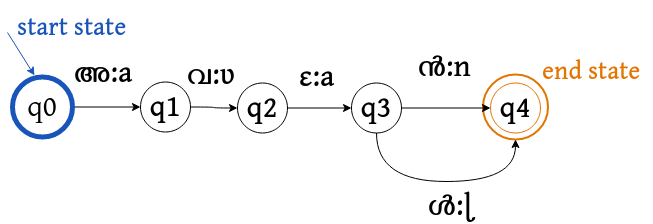
\includegraphics[width=0.7\linewidth]{egfst.png}
	\caption{An FST representing a simple pronunciation mapping that accepts two words {\mal അവൻ} and {\mal  അവൾ}.}
	% 	\Description{Analysis and Surface strings in Phoneme Analyser FST}
	\label{fig:egfst}
\end{figure}


In an FST, every state, \gls{qi}, has a finite  number of transitions to other states. An input and output symbol is used to label each transition. According to the transition function, the FST emits an output symbol for each symbol in the input string after changing its state, starting from the initial state. When it enters the final state, the FST would have accepted every symbol in the input string. The output string is made up of all the emitted symbols at that point \cite{golob2012fst}. For the cases where the number of symbols in input or output strings mismatch, a `null symbol', {\ipa ɛ} is introduced in the transition mapping. 

The FST described in Fig. \ref{fig:egfst}, generates pronunciations for two words {\mal അവൻ} /{\ipa aʋan}/ and {\mal  അവൾ} /{\ipa aʋaɭ}/. The states are represented as circles and marked with their unique number. The initial state is represented by a bold circle and final states by double circles. An input symbol i and an output symbol o are marked on the corresponding directed arc as i : o.  A special symbol {\ipa ɛ} indicates the generation of an output corresponding to an empty input string. Here the inherent vowel {\ipa a} is inserted at the transition from the state {\ipa q1} to {\ipa q3}. Its parameters are defined in Table \ref{tab:fstparam}.

\begin{table}[ht]
	\centering
	\caption{Parameters of FST illustrated in Fig. \ref{fig:egfst} is defined in this table.}
	\label{tab:fstparam}
	\begin{tabular}{c|l}
		\hline \hline
		\textbf{Parameters} & \textbf{Definition}                                                                                                             \\ \hline
		q                  & \{{\ipa q0, q1, q2, q3, q4}\}                                                                                                   \\
		\gls{Sigma}           & \{{\mal അ, വ, ൻ, ൾ}, {\ipa ɛ}\}                                                                                                 \\
		$\Gamma$            & \{{\ipa a, ʋ, n, ɭ}\}                                                                                                           \\
		I                   & \{{\ipa q0}\}                                                                                                                   \\
		F                   & \{{\ipa q4}\}                                                                                                                   \\
		$\delta$            & $\delta$({\ipa q0}, {\mal അ}) = {\ipa q1}; $\delta$({\ipa q1}, {\mal വ}) = {\ipa q2}; $\delta$({\ipa q2}, {\ipa ɛ})= {\ipa q3}; \\
		                    & $\delta$({\ipa q3}, {\mal ൻ}) = {\ipa q4};  $\delta$({\ipa q3},{\mal ൾ}) = {\ipa q4}                                            \\

		$\sigma$            & $\sigma$({\ipa q0}, {\mal അ}) = {\ipa a}; $\sigma$({\ipa q1}, {\mal വ}) = {\ipa ʋ}; $\sigma$({\ipa q2}, {\ipa ɛ})= {\ipa a};    \\
		                    & $\sigma$({\ipa q3}, {\mal ൻ}) = {\ipa n};  $\sigma$({\ipa q3},{\mal ൾ}) = {\ipa ɭ}                                              \\
		\hline

	\end{tabular}

\end{table}

FSTs satisfy closure property, such that the inversion and composition of
transducers are two natural consequences. According to the composition
property, if transducer $T_1$ maps from input symbols $I_1$ to output symbols
$O_1$ and transducer $T_2$ maps from $O_1$ to $O_2$, then the composition $T_1
	|| T_2 $ maps from $I_1$ to $O_2$ \cite{jurafsky2014speech}. The composition of
a series of transducers perform the mapping from an input string to output
string, passing through the states defined by the constituting transducers. The
inversion, $T^{-1}$ of a transducer $T$, reverses the input and output symbols.
This inversion property has enabled the development of Mlphon as a
bidirectional \gls{g2p} converter.

Mlphon, the tool we introduce is developed using SFST. SFST is programming
language for FSTs, written in C++ language \cite{schmid2005programming}. It has
a user-friendly Python API\footnote{SFST Python library:
	\url{https://pypi.org/project/sfst/}}, freely available under the GNU public
license. SFST provides efficient mechanisms for defining the input and output
symbol sets for FSTs and the rules for contextually mapping an input string to
output string. SFST has been employed in the development of state of the art
morphological analysers for Turkish \cite{kayabacs2019trmor}, German
\cite{schmid-etal-2004-smor}, Latin \cite{springmann2016latmor} and Malayalam
\cite{thottingal2019finite}.

The ruleset of Mlphon can be adapted with the necessary script modifications to
other Dravidian languages with a similar script nature. The rulesets and
graphemes must be adjusted to fit the target language. To enable this, we have
made sure the source code is accessible, well-documented, and freely licensed
to allow for adaptations\footnote{https://github.com/kavyamanohar/mlphon}. 
% In a code switching context, a language detector may be needed to separate the text and route it to language-specific g2p systems.

% According to the composition property of FST, if transducer $T_1$ maps from states $I_1$ to $O_1$ and transducer $T_2$ maps from states $O_1$ to $O_2$, then the composition $T_1 \circ T_2 $ maps from $I_1$ to $O_2$. 
% For example, the Syllabifier FST is designed as the composition of three FSTs that perform (i) normalization, (ii) word boundary tagging, and (iii) syllable boundary tagging.

% Parsing grapheme sequence to obtain the phonemes along with their closest articulatory features is referred as forward direction of parsing. The composition of a series of transducers perform the mapping from the input string to the output string, passing through the states defined by the constituting transducers.  The inversion, $T^{-1}$ of a transducer $T$, maps the output symbols of $T$ to its input symbols \cite{jurafsky2014speech}. This inversion property has enabled the  development of Mlphon as a bidirectional grapheme-phoneme converter.

\section{Architectural Description}

\begin{figure}[!ht]
	\centering
	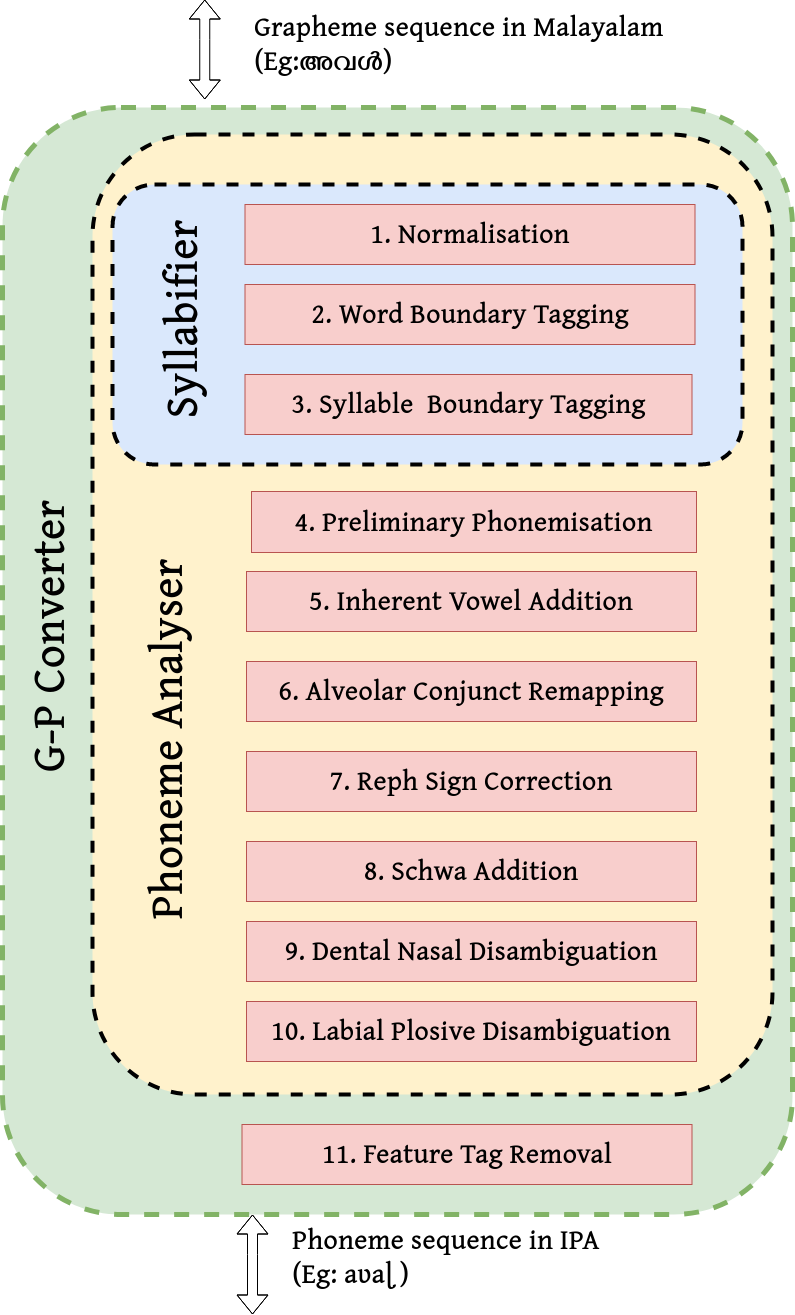
\includegraphics[width=0.6\linewidth]{g2p.png}
	\caption{The system architecture of Mlphon}
	% \Description{Architecture of mlphon described as a flow graph}
	\label{architecture}
\end{figure}

The system architecture of Mlphon is described in Fig. \ref{architecture}. We
follow a modular approach in the design of Mlphon. The mapping from Malayalam
script to IPA is carried out in eleven steps, where each step represents an
FST. In Mlphon, FST parameters are not directly defined. They are instead
compiled from SFST programs. An SFST program is essentially a regular
expression. They represent context sensitive rewrite rules. When the programs
are compiled, we get eleven transducers shown in the architectural diagram in
Fig. \ref{architecture}. Each solid rectangular box in this figure represents an FST that maps between two sets of symbols. They are composed at compile time to give final FSTs in dotted rectangular boxes. Mlphon Python library provides programmable access to these final FSTs.

The SFST programs corresponding to the transducers are simplified and described
in Algorithms \ref{alg:syllabifier} - \ref{alg:disambiguation2}. In the algorithmic
description we use the SFST syntax, where {\ipa '|'} indicates the union
operation, {\ipa '||'} indicates composition operation, '$\leftarrow$'
indicates the mapping of the right hand side input symbol sequence to left hand
side output symbol sequence. They are represented in the form: D $\leftarrow$
[A] B [C], where B is the input with an optional left context A and a right
context C, being mapped to the output D. A, B, C, and D can represent a single
symbol or a sequence of symbols. The individual symbols in a sequence is
separated by a {\ipa '+'}, for enhanced readability.

For transducers that carry out complex tasks, the expressions might be quite
complicated. In order to create complex expressions from simpler ones,
variables are defined \cite{schmid2005sfst}. The SFST program is structured as
a combination of (i) one-to-one and one-to-many mappings from input symbols to
output symbols, (ii) contextual mappings of input symbol sequence to output
symbol sequence, and (iii) self mappings where input symbols are passed as such
to the output. Additional information is provided in comments in the
algorithmic description.
% The input and output symbols of each of these FSTs are listed in Table \ref{alphabets}. 
The individual FSTs are composed at compile time to the final FST structures
namely:

\begin{enumerate}
	\item Syllabifier
	\item Phoneme analyser
	\item Grapheme-Phoneme (G-P) converter
\end{enumerate}

These three FSTs are bundled into Mlphon Python library along with various
utility functions and released under MIT license. The programmable Python API
enables its integration with many downstream NLP tasks as demonstrated in
section \ref{applications}. The functionalities of the individual FSTs are
described in sections \ref{normalisation} to \ref{tagremoval)}. Wherever it is
essential to communicate the functionality, state transitions in each FST are
diagrammatically represented.

% \begin{table*}[!h]
% \begin{center}
%     \begin{minipage}{\textwidth}

% \caption{Input and output symbols of different FSTs}    \label{alphabets}

%     			\setcounter{mpfootnote}{\value{footnote}}
% 			% Redefine the command that produces the footnote number
% 			\renewcommand{\thempfootnote}{\arabic{mpfootnote}}
% \begin{tabular}{clll}
% \hline \hline
%    No. & \textbf{FST}            & \textbf{Input Symbols, \boldmath{$\Sigma$}} & \textbf{Output Symbols, \boldmath{$\Gamma$}} \\\hline
%     1& Normalisation          & Malayalam characters                           &   \textit{Input Symbols}                          \\
%     \rowcolor{Gray}
%     2&Word Boundary Tagging   & Malayalam characters                           &  \textit{Input Symbols} , Word Tags\footnotemark[1] \\
%     3&Syllable Boundary Tagging& Malayalam characters, Word Tags      &  \textit{Input Symbols} , Syllable Tags\footnotemark[2] \\
%     \rowcolor{Gray}
%     4& Preliminary Phonemisation& Malayalam characters,Word Tags, Syllable Tags & IPA characters,  Word Tags, Syllable Tags, \\
%         \rowcolor{Gray}
%     && & Phonemic Feature Tags\footnotemark[3], Graphemic Feature Tags\footnotemark[4] \\
%     5& Inherent Vowel Addition   &  IPA characters,  Word Tags, Syllable Tags &\textit{Input Symbols}, {\ipa <inherentvowel>}  \\
%     \rowcolor{Gray}
%    6&Alveolar Conjuncts Remapping& IPA characters,  Word Tags, Syllable Tags, & \textit{Input Symbols}\\
%     \rowcolor{Gray}
%     7& Reph Sign Correction                           & Phonemic Feature Tags, Graphemic Feature Tags, &\\
%         \rowcolor{Gray}
%     &&                          {\ipa <inherentvowel>} & \\
%     8& Schwa Addition (Samvruthokaram) & IPA characters,  Word Tags, Syllable Tags, & \textit{Input Symbols}, {\ipa <schwa>}  \\
%     &&                                  Phonemic Feature Tags, Graphemic Feature Tags,& \\
%     && {\ipa <inherentvowel>}                                                       &      \\    
%            \rowcolor{Gray}
%    9& Dental Nasal Disambiguation & IPA characters,  Word Tags, Syllable Tags, & \textit{Input symbols}\\
%    \rowcolor{Gray}
%    &&                                  Phonemic Feature Tags, Graphemic Feature Tags,& \\
%   \rowcolor{Gray}
%    && {\ipa <inherentvowel>, <schwa>}                                                       &       \\  
%     10& Labial Plosive Disambiguation & IPA characters,  Word Tags, Syllable Tags, & \textit{Input Symbols}\\
%    &&                                  Phonemic Feature Tags, Graphemic Feature Tags,& \\
%    && {\ipa <inherentvowel>, <schwa>}                                                       &       \\     
%    \rowcolor{Gray}
%    11& Feature Tag Removal & IPA characters,  Word Tags, Syllable Tags, & IPA characters\\
%    \rowcolor{Gray}
%   &&                                  Phonemic Feature Tags, Graphemic Feature Tags,& \\
%    \rowcolor{Gray}
%   && {\ipa <inherentvowel><schwa>}                                                       &       \\        
%    \hline
% \end{tabular}
% 			\footnotetext[1]{{\ipa <BoW> <EoW>} }
% 			\footnotetext[2]{{\ipa <BoS> <EoS> }}
% 			\footnotetext[3]{{\ipa <velar><palatal><dental><retroflex><alveolar><labial><labiodental><plosive><voiceless><voiced><unaspirated><nasal><fricative><flapped> <aspirated><lateral><approximant><glide><trill><glottal><retroflex>}}
%    			\footnotetext[4]{{\ipa <vowel> <v\_sign> <virama><visarga><anuswara><schwa><dotreph><reph><chil> <zwj> <zwnj>} }
% 			\setcounter{footnote}{\value{mpfootnote}}

% 		\end{minipage}
% 	\end{center}
% \end{table*}

% The Mlphon python library (\url{https://pypi.org/project/mlphon/}) provides programmable access to Syllabifier, Phoneme Analyser and G-P Converter

% Table \ref{alphabets} shows the symbol set of different FSTs in Mlphon. The rules for mapping between them are defined in Algorithms \ref{syllabifier}-\ref{disambiguation2}. During compilation, the symbols and the rules get converted into FSTs with internally formulated states and transition functions. 

% \begin{figure*}[!h]
% 	\centering
% 	\includegraphics[width=0.9\linewidth,height=0.75\textheight]{architecture.png}
% 	\caption{The system architecture of Mlphon. Each solid rectangular box represents an FST that maps between two sets of symbols. They are composed at compile time to give final FSTs in dotted rectangular boxes. Mlphon python library provides programmable access to these final FSTs.}
% 	% \Description{Architecture of mlphon described as a flow graph}
% 	\label{architecture}
% \end{figure*}

% \begin{table*}[]
%     \centering
%         \caption{Input and output symbols of different FSTs}
%     \label{alphabets}
% \begin{tabular}{|c|l|l|}
% \hline \hline
%     \textbf{FST} & \textbf{Input Alphabets, \boldmath{$\Sigma$}} & \textbf{Output Alphabets, \boldmath{$\Gamma$}} \\\hline
%    \multirow{8}{*}{ Syllabifier} &{\mal അ ആ ഇ ഈ ഉ ഊ ഋ ൠ ഌ ൡ എ ഏ ഐ ഒ ഓ ഔ} & {\mal അ ആ ഇ ഈ ഉ ഊ ഋ ൠ ഐ ഒ ഓ ഔ}\\
%     &{\mal ാ ി ീ ൢ ൢ ു ൂ ൃ ൄ ൢ ൣ െ േ ൈ ൊ } &{\mal ാ ി ീ ൢ ൢ ു ൂ ൃ ൄ ൢ ൣ െ േ ൈ ൊ } \\
%         &{\mal ോ ൗ ൌ ം  ഃ ് ൎ} &{\mal ോ ൗ ൌ ം  ഃ ് ൎ} \\
%     &{\mal ക ഖ ഗ ഘ ങ ച ഛ ജ ഝ ഞ ട ഠ ഡ ഢ ണ }& {\mal ക ഖ ഗ ഘ ങ ച ഛ ജ ഝ ഞ ട ഠ ഡ ഢ ണ }\\
%         &{\mal  ഺ ഩ ത ഥ ദ ധ ന പ ഫ ബ ഭ മ}& {\mal ഺ ഩ ത ഥ ദ ധ ന പ ഫ ബ ഭ മ}\\
%         &{\mal  യ ര ല വ ശ ഷ സ ഹ ള ഴ റ ൺ ൻ ർ ൽ ൾ ൿ ൔ ൕ ൖ}& {\mal യ ര ല വ ശ ഷ സ ഹ ള ഴ റ ൺ ൻ ർ ൽ ൾ ൿ ൔ ൕ ൖ}\\
%         && {\ipa <BoS> <EoS>}\\
%         & \textbf{Eg Input}: {\mal വള} & \textbf{Eg Output}:  {\ipa <BoS>}{\mal വ}{\ipa <EoS>}{\ipa< BoS>} {\mal ള}{\ipa <EoS> } \\
%     \hline
%      &{\mal അ ആ ഇ ഈ ഉ ഊ ഋ ൠ ഌ ൡ എ ഏ ഐ ഒ ഓ ഔ} & {\ipa  ə
% a aː i iː u uː rɨ rɨː lɨ lɨː e eː ai̯ o oː au̯
% k kʰ ɡ ɡʱ ŋ
% t͡ʃ t͡ʃʰ ɟ ɟʱ ɲ
% }\\

%      &{\mal ാ ി ീ ൢ ൢ ു ൂ ൃ ൄ ൢ ൣ െ േ ൈ ൊ } &{\ipa ʈ ʈʰ ɖ ɖʱ ɳ
% t̪ t̪ʰ d̪ d̪ʱ n̪
% ṯ n
% p pʰ b bʱ m
% j ɾ l ʋ ʃ ʂ s ɦ ɭ ɻ r f} \\

%     & {\mal ോ ൗ ൌ ം  ഃ ് ൎ}& {\ipa <vowel> <v\_sign> <virama><visarga><anuswara> }\\

%         &{\mal ക ഖ ഗ ഘ ങ ച ഛ ജ ഝ ഞ ട ഠ ഡ ഢ ണ }&{\ipa <schwa><dotreph><velar><palatal><dental>} \\
%         &{\mal  ഺ ഩ ത ഥ ദ ധ ന പ ഫ ബ ഭ മ}&{\ipa <retroflex><alveolar><labial><labiodental> } \\
% Phoneme    &{\mal  യ ര ല വ ശ ഷ സ ഹ ള ഴ റ ൺ ൻ ർ ൽ ൾ ൿ ൔ ൕ ൖ}&{\ipa <plosive> <voiceless> <voiced><aspirated>} \\
%      Analyser    &&{\ipa <unaspirated><nasal><fricative><flapped> } \\
%          &&{\ipa <lateral><approximant><glide><trill>} \\
%          &&{\ipa <glottal><retroflex>} \\
%          &&{\ipa <reph><chil> <zwj> <zwnj><inherentvowel>} \\
% & \textbf{Eg Input}: {\mal വള}  & \textbf{Eg Output}: {\ipa <BoS>}{\ipa ʋ}{\ipa <approximant><labiodental>}\\
% && {\ipa a}{\ipa <inherentvowel><EoS><BoS>}{\ipa ɭ}{\ipa <lateral>}\\
% &&{\ipa <retroflex>}{\ipa a}{\ipa <inherentvowel><EoS>} \\   \hline
%         &{\mal അ ആ ഇ ഈ ഉ ഊ ഋ ൠ ഌ ൡ എ ഏ ഐ ഒ ഓ ഔ} & {\ipa  ə
% a aː i iː u uː rɨ rɨː lɨ lɨː e eː ai̯ o oː au̯
% k kʰ ɡ ɡʱ ŋ
% t͡ʃ t͡ʃʰ ɟ ɟʱ ɲ
% }\\

%      &{\mal ാ ി ീ ൢ ൢ ു ൂ ൃ ൄ ൢ ൣ െ േ ൈ ൊ } &{\ipa ʈ ʈʰ ɖ ɖʱ ɳ
% t̪ t̪ʰ d̪ d̪ʱ n̪
% ṯ n
% p pʰ b bʱ m
% j ɾ l ʋ ʃ ʂ s ɦ ɭ ɻ r f} \\
%   &{\mal ോ ൗ ൌ ം  ഃ ് ൎ} &\\
%   G-P  &{\mal ക ഖ ഗ ഘ ങ ച ഛ ജ ഝ ഞ ട ഠ ഡ ഢ ണ }&\\

%  Converter &{\mal  ഺ ഩ ത ഥ ദ ധ ന പ ഫ ബ ഭ മ} &\\
%   &{\mal  യ ര ല വ ശ ഷ സ ഹ ള ഴ റ ൺ ൻ ർ ൽ ൾ ൿ ൔ ൕ ൖ}&\\
% &\textbf{Eg. Input}:{\mal വള} & \textbf{ Eg. Output}: {\ipa ʋaɭa} \\

%    \hline
% \end{tabular}

% \end{table*}

%See Fig. \ref{fstbox}, showing an example of analysis and surface strings of Phoneme Analyser FST.

%\begin{figure}[h]
%	\centering
%	\includegraphics[width=0.9\linewidth]{FSTbox.pdf}
%	\caption{Analysis and Surface strings in Phoneme Analyser FST}
%	% \Description{Analysis and Surface strings in Phoneme Analyser FST}
%	\label{fstbox}
%\end{figure}

% \subsection{Syllabifier FST}
% \label{syllabification}

\subsection{Normalisation}
\label{normalisation}

This FST accepts all Malayalam characters and invisible zero width
characters\footnote{Zero Width Joiner:
	\url{https://en.wikipedia.org/wiki/Zero-width_joiner}}. Characters that do not
require normalisation are self mapped. Character sequences that essentially
represents the same graphemes are normalised to a standard form.

\begin{figure}[htpb]
	\centering
	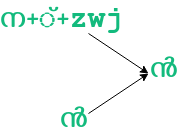
\includegraphics[width=0.25\linewidth]{norm.drawio.png}
	\caption{Two alternate representations of {\mal ൻ} at input is being mapped to the normalised form at the output.}
	% 	\Description{Analysis and Surface strings in Phoneme Analyser FST}
	\label{fig:norm}
\end{figure}

Specifically this FST converts chillus represented as the sequence \texttt{base
	consonant}, \textit{virama} ({\mal ്}), \texttt{zwj} to atomic forms as shown in Fig. \ref{fig:norm}. It also converts {\mal ന്റ} {\ipa /nṯa/} represented as the sequence [{\mal ൻ},
\textit{virama} ({\mal ്}), {\mal റ}] to [{\mal ന}, \textit{virama} ({\mal ്}),
{\mal റ}]. Fig. \ref{fig:egnorm} provides an example indicating the state
transitions happening in an FST that performs this.  The word final \textit{chillu} grapheme represented as {\mal ന, ്,} \texttt{zwj} is normalised to a common form of single atomic character, {\mal ൻ},  by passing through states from q2 , q3, q4 and q5. If the word were already in normalised form, that character is self mapped as indicated in other transitions. The procedural description is provided in Algorithm \ref{alg:syllabifier}.

%The entire alphabet of Malayalam is defined as a self mapping transducer.

\begin{figure}[htpb]
	\centering
	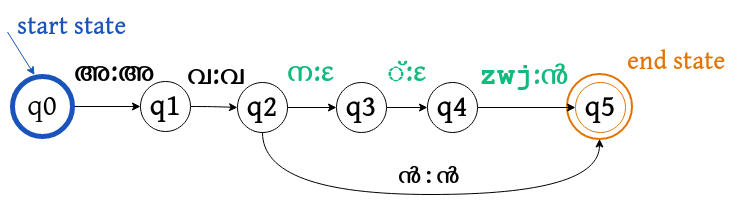
\includegraphics[width=0.8\linewidth]{egs_norm.png}
	\caption{Normalisation of the word {\mal അവൻ}, indicating the two possible input sequences generating the normalised output.}
	% 	\Description{Analysis and Surface strings in Phoneme Analyser FST}
	\label{fig:egnorm}
\end{figure}

\subsection{Word Boundary Tagging}

This FST accepts all Malayalam characters. The token passed to Mlphon for
analysis is considered as a word. Tags in angle brackets {\ipa \gls{bow}} and {\ipa
		\gls{eow}} are added to indicate the beginning of word and the end of word
respectively by this FST and is returned to the output. The procedural
description is provided in Algorithm \ref{alg:syllabifier}.

\subsection{Syllable Boundary Tagging}
\label{syllabletagger}

\begin{figure}[htpb]
	\centering
	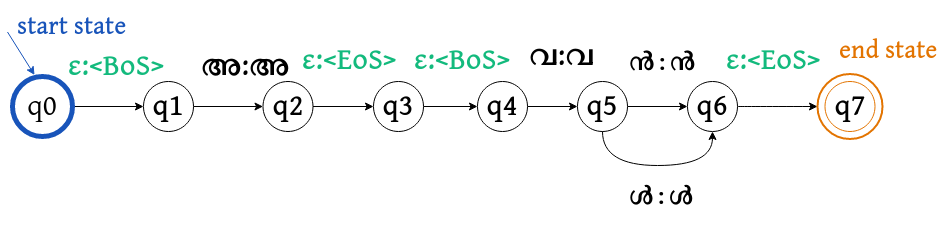
\includegraphics[width=0.9\linewidth]{g2p-syltags.png}
	\caption{Insertion of syllable tags, {\ipa \gls{bos} \gls{eos}} are indicated by transitions in green colour. All other symbols are mapped to themselves. Word boundary tags inserted in previous FST is also shown. }
	% 	\Description{Analysis and Surface strings in Phoneme Analyser FST}
	\label{fig:g2p-syltags}
\end{figure}
This FST accepts all Malayalam characters, along with word boundary tags. As discussed in section  \ref{syllablestructure}, some character sequences are invalid according to Malayalam script grammar. The syllabifier FST checks for validity of character sequences to form syllables.  An invalid sequence of Malayalam characters will  not find a path from the start state of this FST to the end state and will summarily be rejected. On valid input strings, it inserts tags - {\ipa \gls{bos}}, {\ipa \gls{eos}} - at appropriate positions to indicate the beginning and end of the syllables. The syllable boundary tags are essential for pronunciation analysis. This procedure is explained in Algorithm \ref{alg:syllabifier}. An example for the insertion of syllable tags is indicated in Fig. \ref{fig:g2p-syltags}.

\begin{algorithm}[htpb]
	\caption{Normalisation, Word Boundary Tagging, Syllable Boundary Tagging}\label{alg:syllabifier}
	\begin{algorithmic}[1]
	\Procedure{Normalisation}{}
		\State \texttt{chillunorm\_fst}: {\ipa chillu} $\gets$ {\ipa base consonant+virama+zwj} \Comment{Define a named FST for chillu normalisation}
		\State \texttt{ntanorm\_fst}: {\mal ന+്+റ} $\gets$ {\mal ൻ+്+റ}
		\State \Return \texttt{chillunorm\_fst} {\ipa  | } \texttt{ntanorm\_fst} \Comment{It is the union of two predefined FSTs}
	\EndProcedure
	\Procedure{Word Boundary Tagging}{}
		\State \Return {\ipa <BoW>+token+<EoW>} $\gets$ {\ipa token} \Comment{Insert boundary tags to input word token}
	\EndProcedure
	\Procedure{Syllable boundary tagging}{}
 		\State {\ipa c\_v} $\gets$ {\ipa consonant + virama}
   		\State {\ipa syl\_end} $=$ {\ipa [anuswara, visarga, chillu]}  \Comment{syl\_end is a variable, that can take any value in the list}
        \State \Comment{Four types of character sequences that constitute a syllable is defined in the following lines}
		\State {\ipa Type 1} $\gets$ {\ipa <BoW>+vowel+syl\_end?}  \Comment{? indicates optionaity}
		\State {\ipa Type 2} $\gets$ {\ipa consonant+vowelsign?+syl\_end?}
		\State {\ipa Type 3} $\gets$ {\ipa c\_v * + consonant} \Comment{* indicates one or more occurence}
		\State {\ipa Type 4} $\gets$ {\ipa c\_v ? + consonant + {\mal ു}? + virama + <EoW>}
		\State {\ipa syllable} $\gets$ {\ipa Type 1 | Type 2 | Type 3 | Type 4 } \Comment{A syllable is any of the 4 types}
		\State \Return {\ipa <BoS> + syllable +  <EoS>} $\gets$ {\ipa syllable} \Comment{Insert boundary tags to syllables}
	\EndProcedure
% 	\State \texttt{Syllabifier}: \texttt{Normalizer} $\circ$ \texttt{WordBoundaryTagger} $\circ$ \texttt{SyllableBoundaryTagger}
	\end{algorithmic}
\end{algorithm}



\subsection{Preliminary Phonemisation}

This FST accepts valid sequence of Malayalam characters separated by word and
syllable boundary tags. The transitions defined by this FST maps every grapheme
to phonemes as per tables in Appendix \ref{app:app1} \ref{vowelgrapheme}-\ref{chillus} along with phonetic
or graphemic feature tags.
% The list of these tags are available in Table \ref{alphabets}. 
The preliminary mapping carried out by this FST will be modified by subsequent
FSTs based on contexts. The boundary tags are self mapped, so that they will be
retained as such in the output. An example of mapping the graphemes {\mal സ}
and {\mal മ} to its phoneme with phonetic features is described in Algorithm
\ref{alg:tagging}.

\begin{algorithm}[htpb]
	\caption{Preliminary Phonemisation}\label{alg:tagging}
	\begin{algorithmic}[1]
	\Procedure{Preliminary Phonemisation}{}
		\State \texttt{g2p\_1}: {\ipa s+<fricative>+<alveolar>} $\gets$ {\mal സ}
		\State  \texttt{g2p\_2}: {\ipa m+<labial>+<nasal>} $\gets$ {\mal മ} 
		\State ...
		\State ... \Comment Basic G2P mappings
		\State \Return \texttt{g2p\_1} $||$ \texttt{g2p\_1} . . . 
  \State \Comment Composition of basic G2P mappings
	\EndProcedure
	\end{algorithmic}
\end{algorithm}


% The preliminary mapping of graphemes , are performed by this FST. During this mapping,  phonetic feature tags are added to each  phoneme.
% , and vowel phonemes are associated with tags indicating their graphemic origin (independent vowel or vowel sign).
% Once word and syllable boundary tags are inserted, the next task is to map each grapheme to phoneme. This is done as per the mapping listed in Tables  .  Inherent vowels and effect of virama on phonemes will be mapped only in the subsequent stages.

\subsection{Inherent Vowel Addition}

Algorithm \ref{alg:disambiguation} outlines the rules for adding the inherent vowel /a/ after consonant phonemes in certain circumstances. Specifically, if the consonant phoneme is at the end of a syllable position, or if it is followed by the \textit{anuswara}, \textit{visarga}, or a \textit{chillu}, then the inherent vowel /a/ is added.

\subsection{Alveolar Conjuncts Remapping}

The alveolar consonant clusters {\mal ന്റ} {\ipa /nṯa/} and {\mal റ്റ} {\ipa /ṯṯa/} are composed of the dental nasal {\mal ന} {\ipa /n̪a/} and the alveolar trill {\mal റ} {\ipa /ra/}, which have distinct pronunciations. Therefore, the grapheme sequence  {\mal ന} {\ipa /n̪a/} followed by a virama and {\mal റ} {\ipa /ra/} can be mapped to  {\ipa /nṯa/} instead of {\ipa /n̪ra/}. Similarly, the grapheme sequence {\mal റ} {\ipa /ra/} followed by a virama and {\mal റ} {\ipa /ra/} can be mapped to {\ipa /ṯṯa/} instead of {\ipa /rra/}. To achieve this unambiguous mapping, an FST is used to check the context and remap these phonemes, as described in Algorithm \ref{alg:disambiguation}.


% The most common alveolar consonant clusters in Malayalam, {\mal ന്റ} {\ipa
% 		/nṯa/} and {\mal റ്റ} {\ipa /ṯṯa/} are constituted from consonants dental nasal
% 	{\mal ന} /{\ipa n̪a/} and alveolar trill {\mal റ} {\ipa /ra/}, the
% pronunciations of which are strikingly different. Thus the grapheme sequence
% 	{\mal ന} {\ipa /n̪a/}, \textit{virama}, {\mal റ} {\ipa /ra/} can be mapped to
% 	{\ipa /nṯa/} instead of {\ipa /n̪ra/}. Also the grapheme sequence {\mal റ} {\ipa
% 		/ra/}, \textit{virama}, {\mal റ} {\ipa /ra/} can be mapped to {\ipa /ṯṯa/}
% instead of {\ipa /rra/}. This unambiguous mapping is done by an FST that checks
% the context and remaps these phonemes as indicated in Algorithm
% \ref{alg:disambiguation}.

\subsection{Reph Sign Correction}

If the final consonant in a cluster is the alveolar tap {\mal ര} {\ipa /ɾa/},
its pronunciation gets modified to {\mal റ} {\ipa /ra/} depending on the
preceding consonants. The {\mal ര} {\ipa /ɾa/} sound is retained only if the
preceding consonant of the cluster is voiced velar or dental plosive ({\mal ഗ}
	{\ipa /ga/} or {\mal ദ} {\ipa /d̪a/}) as described in Algorithm
\ref{alg:disambiguation}.


\begin{algorithm}[htpb]
	\caption{Inherent Vowel Addition, Alveolar Conjuncts Remapping and Reph Sign Correction}\label{alg:disambiguation}
	\begin{algorithmic}[1]
	\Procedure{Inherent Vowel Addition}{}
        \State {\ipa pre\_context} $=$ {\ipa consonant+<tags>} \Comment{Define a variable that is a sequence of consonants and tags}
		\State {\ipa post\_context} $=$ {\ipa [<chil>, <anuswara>, <visarga>, <EoS>]} \Comment{Define a variable that takes any value in the list}
		\State \Return {\ipa [pre\_context]} {\ipa a+<inherentvowel>} {\ipa [post\_context]} $\gets$ {\ipa [pre\_context]}  {\ipa ɛ } {\ipa [post\_context]}
	\EndProcedure  \Comment <tags> - represent the sequence of phonetic feature tags
		\Procedure{Alveolar conjuncts remapping}{}
		\State \texttt{tta\_fst}: {\ipa [<BoS>,<virama>]+ṯ+<tags>+ṯ+<tags>} $\gets$ {\ipa [<BoS>,<virama>]+r+<tags>+r+<tags>}
		\State \texttt{nta\_fst}: {\ipa <BoS>+n̪+<tags>+ṯ+<tags>} $\gets$ {\ipa <BoS>+n+<tags>+r+<tags>}
		\State \Return \texttt{tta\_fst $||$ nta\_fst} \Comment{Composition of two FSTs}
		\EndProcedure
	\Procedure{Reph Sign Correction}{}
		\State \Return {\ipa [ɡ,d̪]+<tags>+<virama>+ɾ+<flapped>+<reph>} $\gets$ {\ipa [ɡ,d̪]+<tags>+<virama>+r+<trill>+<reph>}
	\EndProcedure
	\end{algorithmic}
\end{algorithm}


\subsection{Schwa Addition (\textit{Samvruthokaram})}

\textit{Samvruthokaram} is a unique feature of Malayalam. Whenever there are consonants followed by \textit{virama} at word ends, a half-u sound of mid-central vowel schwa is added at word end as described in Algorithm \ref{alg:disambiguation2}. This FST basically disambiguates the function of \textit{virama}. Loan words get adapted to native pronunciation by schwa addition at word ends. eg: {\mal ബാങ്ക്} {\ipa /baːŋkə/} (\textit{bank)}

% But there are non-native proper names, derived from Sanskrit or other foreign language, that end in virama, but pronunciation involves no schwa. eg: ജോർജ്, സന്തോഷ്, രാജീവ്, ജോസ്

% But there are non-native proper names, derived from Sanskrit or other foreign language, that end in virama, but pronunciation involves no schwa. eg: ജോർജ്, സന്തോഷ്, രാജീവ്, ജോസ്

\subsection{Dental Nasal Disambiguation}

% As already discussed in Section \ref{consonantg2p}, the alveolar nasal grapheme {\mal ഩ} {\ipa /na/}, is not widely used in Malayalam except in the context of grammatical discussions. 
The dental nasal grapheme {\mal ന} {\ipa /n̪a/}, is pronounced as the alveolar
nasal {\ipa /na/} in the following contexts\cite{prabo2016}:
% and is mostly in unambiguous distribution in native Malayalam morphemes. The contexts in which {\mal ന} {\ipa /n̪a/} takes alveolar {\ipa /na/} pronunciation 

\begin{enumerate}
	\item When a morpheme medial syllable starts in {\mal ന} and is followed by a vowel
	      sound.

	      eg: {\mal ആന} {\ipa /aːna/} (\textit{elephant}), {\mal ഗാനം} {\ipa /ɡaːnam/}
	      (\textit{song}), {\mal അനുജൻ} {\ipa /anuɟan/} (\textit{younger brother})
	\item When {\mal ന} is the starting character in a consonant cluster followed by
		      {\mal യ} {\ipa /ja/}, {\mal വ} {\ipa /ʋa/} or {\mal മ} {\ipa /ma/}.

	      eg: {\mal നന്മ} {\ipa /n̪anma/} (\textit{virtue}), {\mal ന്യായം} {\ipa /njaːjam/}
	      (\textit{justice}), {\mal അന്വേഷണം} {\ipa /anʋeːʂaɳam/ }(\textit{enquiry})
	\item When {\mal ന} is the second character in a consonant cluster, beginning with
		      {\mal ക} {\ipa /ka/}, {\mal ഘ} {\ipa /ɡʱa/}, {\mal പ} {\ipa /pa/}, {\mal മ}
		      {\ipa /ma/}, {\mal ശ} {\ipa /ʃa/} and {\mal സ} {\ipa /sa/}.

	      eg: {\mal വിഘ്നം} {\ipa /ʋiɡʱnam/} (\textit{blockage}) , {\mal സ്വപ്നം} {\ipa
			      /sʋapnam/} (\textit{dream}), {\mal പ്രശ്നം} {\ipa /praʃnam/} (\textit{issue}),
	      {\mal സ്നേഹം} {\ipa /sneːɦam/} (\textit{love})

\end{enumerate}

These three rules are implemented by identifying the context of appearance of
	{\mal ന} in terms of the surrounding consonants and syllable boundaries etc. as
described in the Algorithm \ref{alg:disambiguation2}.

%
%As the tool can not detect presence of multiple morphemes from a morphologically complex word, word-medial morpheme beginning with {\mal ന} will be identified as {\ipa n<nasal><alveolar>} instead of {\ipa n̪<nasal><dental>} as in the transcription of {\mal സേവ\textbf{നാ}ഴി} {\ipa /seːʋanaːɻi/}. The percentage of failures it can cause in g2p mapping is analysed in the evaluation section.
%  The second and third rules describe how to pronounce {\mal ന} when it occurs in consonant clusters. It depends on the preceding or succeeding consonants in the clusters and the distribution is unambiguous.

% When {\mal ന} is geminated, grapheme context and the morphological composition determines the pronunciation. For example, {\mal എന്നാൽ} has two different morphological analysis possible. When it is the instrumental inflection on first person singular in Malayalam, it should be phoneme mapped to {\ipa /ennal/}. When the same word has an alternate usage as `but', its phoneme mapping should be  {\ipa /en̪n̪al/}. Such words are assigned with two possible phonemic mappings. These rules are insufficient to handle loan words and morphologically complex words and causes phoneme transcription errors discussed in Section \ref{goldlexicon}.

%\begin{lstlisting}[frame=tb, language=python, caption= Python script for grapheme to phoneme conversion, label ={g2ppython}]
%	from mlphon import PhoneticAnalyser
%	mlphon = PhoneticAnalyser()
%	print(mlphon.grapheme_to_phoneme('@{\mal വള}@'))
%	print(mlphon.grapheme_to_phoneme('@{\mal അവൻ}@'))
%	['@{\ipa ʋaɭa}@']
%	['@{\ipa aʋan}@']
%\end{lstlisting}

\subsection{Labial Plosive Disambiguation}
\label{labiodentalfricative}

The unvoiced aspirated labial plosive grapheme {\mal ഫ} {\ipa /pʰa/} is used to
represent the labiodental fricative {\ipa /f/} in non-native words. On
analysing a corpus of 100k most frequent Malayalam words
\cite{kunchukuttan2020ai4bharat}, only 6\% of words that contained the letter
	{\mal ഫ} were native. All those native words had the letter {\mal ഫ}, either
preceded by the letter {\mal സ്} or followed by {\mal ല}. This graphemic context
is used as the parameter to determine the word origin and remap fricative to
plosive as described in Algorithm \ref{alg:disambiguation2}.

% Native words with {\mal ഫ} /pʰ/: {\mal ഫലം} {\ipa /pʰalam/} (\textit{fruit}), {\mal ഫലിതം} {\ipa /pʰalit̪am/} (\textit{joke}), {\mal സ്ഫടികം} {\ipa /spʰaʈikam/} (\textit{glass}) . Non-native words with {\mal ഫ} {\ipa /f/}: {\mal ഫാൻ} {\ipa /faːn/}(\textit{fan}) , {\mal ഫോൺ} {\ipa /foːɳ/} (\textit{phone}), {\mal ഫാക്ടറി} {\ipa /faːkʈari/} (\textit{factory}), {\mal ഫാസ്റ്റ്} {\ipa /faːsṯ/ }(\textit{fast}), {\mal ഫാഷൻ} {\ipa /faːʂan/} (\textit{fashion}), {\mal ഇൻഫർമേഷൻ} {\ipa /infarmeːʂan/} (\textit{information}).

% \subsubsection{Phoneme Sequence with Feature Tags}

% The sequence of transducers described above is composed into a single large FST during compile time. Fig. \ref{phanalysissfst} illustrates the state transitions and the insersion of tags in the phoneme analyser FST when input tokens passed are: {\mal വള} and {\mal അവൻ}. The python interface of Mlphon utilizes this FST to phonemically analyse the Malayalam word and return the sequence of phonemes and feature tags. If the token {\mal അവൻ } is passed to the phoneme analyser FST, it returns the string  {\ipa <BoS>a<vowel><EoS><BoS>ʋ<approximant><labiodental>a <inherentvowel>n<chil><EoS>}.

% A tag parser function in the python interface can return the IPA and anaysis tags.

\begin{algorithm}[htpb]
	\caption{Schwa Addition, Dental Nasal Disambiguation,  Labial Plosive Disambiguation}\label{alg:disambiguation2}
	\begin{algorithmic}[1]
	\Procedure{Schwa Addition}{}
		\State \texttt{schwa\_1}: {\ipa ə+<schwa>+<EoS>} $\gets$ {\ipa u+<v\_sign>+<virama>+<EoS>} \Comment{Define named FSTs for schwa addition}
		\State \texttt{schwa\_2}: {\ipa ə+<schwa>+<EoS>} $\gets$ {\ipa <virama>+<EoS>} 
		\State \Return \texttt{schwa\_1} $||$ \texttt{schwa\_2} \Comment{Return the composition of two FSTs}
	\EndProcedure
	\Procedure{Dental Nasal Disambiguation}{}
		\State \texttt{nasalrule\_1}:
		{\ipa <BoS>+n+<alveolar+<virama>+[j,ʋ,m]} $\gets$ {\ipa <BoS>+n̪<dental+<virama>+[j,ʋ,m]} \Comment{Define named FSTs}
		\State \texttt{nasalrule\_2}:
		{\ipa <EoS>+<BoS>+n<alveolar>+[vowel]} $\gets$ {\ipa <EoS>+<BoS>+n̪+<dental+[vowel]}
		\State \texttt{nasalrule\_3}: {\ipa [k,ɡʱ,p,m,ʃ,s]+<tags>+<virama>n<alveolar>} $\gets$ {\ipa [k,ɡʱ,p,m,ʃ,s]+<tags>+<virama>n̪<dental>}
		\State \Return \texttt{nasalrule\_1 $||$ nasalrule\_2 $||$ nasalrule\_3} \Comment{Return the composition of three FSTs}
	\EndProcedure
	\Procedure{Labial Plosive Disambiguation}{}
		\State \texttt{fa\_1}: {\ipa <BoW>+<BoS>+pʰ<plosive>+a+<EoS>+<EoW>} $\gets$ {\ipa <BoW>+<BoS>+f<fricative>>+a+<EoS>+<EoW>}
		\State \texttt{fa\_2}: {\ipa s+<fricative>+<alveolar>+<virama>+pʰ+<plosive>} $\gets$ {\ipa s+<fricative>+<alveolar>+<virama>+f<fricative>}
		\State \texttt{fa\_3}: {\ipa pʰ<plosive>+a+<EoS>+<BoS>+l} $\gets$ {\ipa f<fricative>+a+<EoS>+<BoS>+l}
		\State \Return \texttt{fa\_1 $||$ fa\_2 $||$ fa\_3} \Comment{Return the composition of three FSTs}
	\EndProcedure
	\end{algorithmic}
\end{algorithm}


\subsection{Feature Tag Removal}
\label{tagremoval)}

The tag-removal FST removes the boundary tags and phonetic feature tags, by
mapping them to the null symbol {\ipa ɛ}. It will leave just the IPA symbols at
the output.

\section{Syllabifier FST}
\label{syllabification}

The composition of the series of FSTs from \ref{normalisation} to
\ref{syllabletagger} results in a very useful module that performs
syllabification of Malayalam text. We compose these FSTs to get the Syllabifier
FST and provide programmable access to it in the Mlphon Python library. This
module has interesting applications like developing subword level language
modelling for ASR as described in section \ref{applications}. An illustration of
this module accepting Malayalam text as input and generating output with
syllable boundary tags is shown in Fig. \ref{fig:syllabifierblock}.

\begin{figure}[htpb]
	\begin{center}
		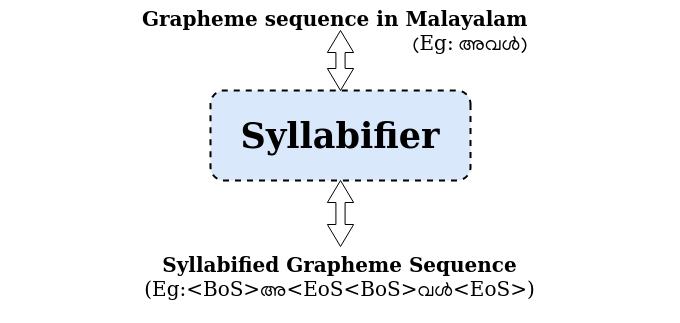
\includegraphics[width=0.7\linewidth]{syllabifier.png}
		\caption{Syllabifier performing syllabification on the word {\mal അവൾ}. Boundary tags for words and syllables are demonstrated.}
		% \Description{State Transition diagram of FST for syllabification}
		\label{fig:syllabifierblock}
	\end{center}

\end{figure}

% \begin{figure*}[!h]
% 	\centering
% 	\includegraphics[width=0.9\linewidth]{syllable-drawio.png}
% 	\caption{State transitions in syllabifier FST, when the input words are  {\mal അവൻ} and {\mal അവൾ}. }
% 	% \Description{State Transition diagram of FST for syllabification}
% 	\label{sylfst}
% \end{figure*}

% Fig. \ref{sylfst} illustrates the state transitions and the insertion of tags in the syllabifier FST when input tokens passed are: {\mal അവൾ} and {\mal അവൻ}. Note that {\ipa ε} indicate the empty transition string. 
If the token passed to the syllabifier is {\mal അവൾ} {\ipa /aʋaɭ/}, it returns the
syllabified string {\ipa <BoS>}{\mal അ}{\ipa <EoS> <BoS>}{\mal വൾ}{\ipa <EoS>}.
The Python interface to the FST for syllabification, parses the boundary tags
and returns the sequence of syllables.
% as shown in the Listing \ref{pythonsyllabification}.

%\begin{lstlisting}[frame=tb,language=python,caption= Python script for phoneme to grapheme conversion, label={p2gpython}]
%	from mlphon import PhoneticAnalyser
%	mlphon = PhoneticAnalyser()
%	print(mlphon.phoneme_to_grapheme('@{\ipa ʋaɭa}@'))
%	print(mlphon.phoneme_to_grapheme('@{\ipa aʋan}@'))
%	['@{\mal വള}@']
%	['@{\mal അവൻ}@']
%\end{lstlisting}

\section{Phoneme Analyser FST}

Phoneme analyser FST is compiled as a composition of 10 FSTs described in
sections \ref{normalisation} to \ref{labiodentalfricative} and indicated in
Fig. \ref{architecture} of Mlphon architecture. This FST accepts a grapheme
sequence as input and returns phoneme sequence, tagged with their phonetic
features. If the token {\mal അവൾ } is passed to the phoneme analyser FST, it
returns the string {\ipa <BoS>a<vowel><EoS><BoS>ʋ<approximant><labiodental>a
		<inherentvowel>ɭ<chil><EoS>} as illustrated in Fig. \ref{fig:analysisblock}. This
module can play crucial role in the context of linguistic learning providing
pronunciation information regarding the graphemes in a word.

% Its operation as the composition of different FSTs is explained in the following subsections.
% The sequence of transducers  is composed into a single large FST during compile time. 
\begin{figure}[htpb]
	\centering
	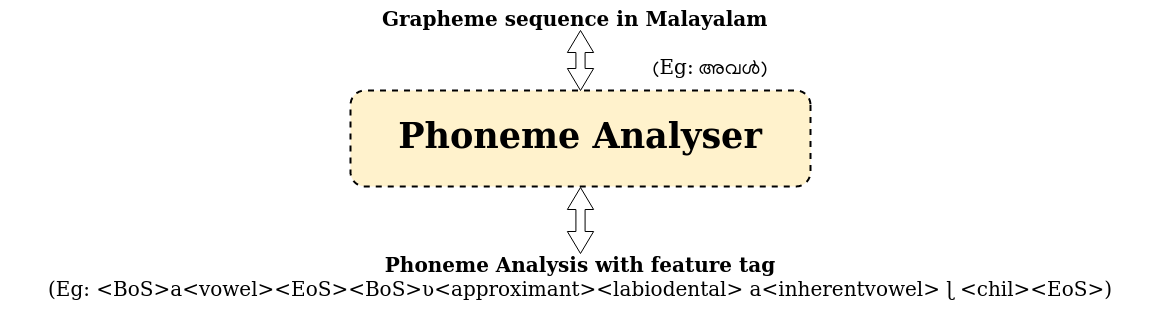
\includegraphics[width=0.9\linewidth]{phonemeanalyser.png}%{analysisbox-drawio.png}
	\caption{Phoneme analyser performing analysis on the word {\mal അവൾ}. It returns the sequence of phonemes in its pronunciation along with articulatory feature tags in angle brackets.}
	% \Description{State Transition diagram of FST for syllabification}
	\label{fig:analysisblock}
\end{figure}

Fig. \ref{phanalysissfst} illustrates the state transitions and the insertion
of tags in the phoneme analyser FST when input tokens passed are: {\mal അവൾ} {\ipa /aʋaɭ/} and {\mal അവൻ} {\ipa /aʋan}/. The Python interface of Mlphon utilises this FST to analyse the Malayalam word and return the sequence of phonemes and phonetic feature tags like place and manner of articulation.

\begin{figure}[htpb]
	\centering
	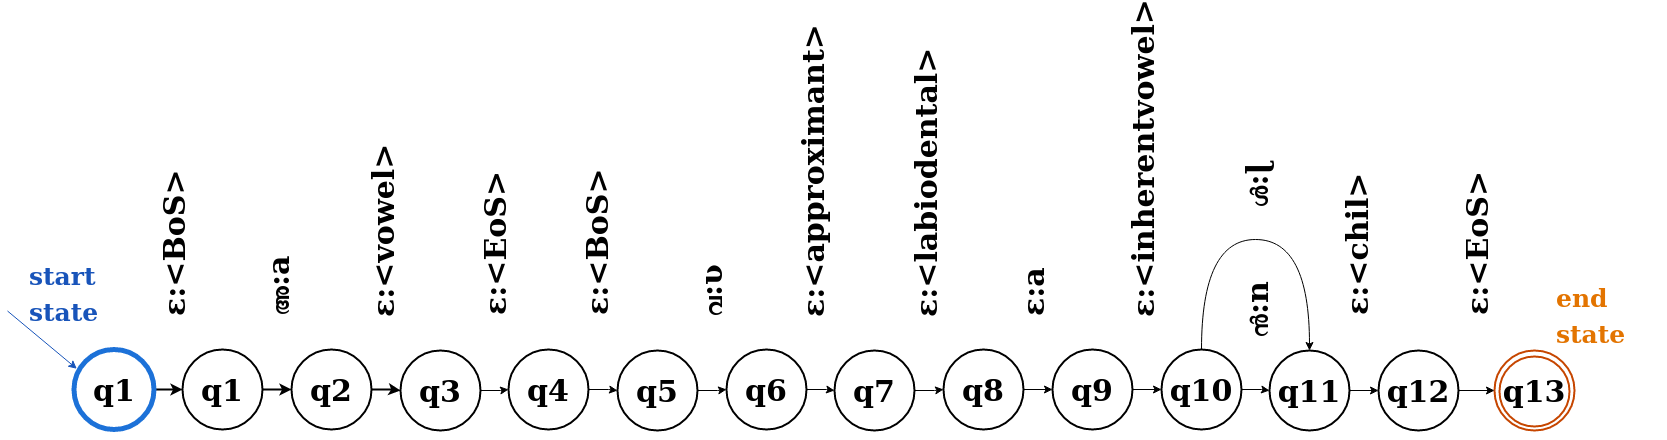
\includegraphics[width=\linewidth]{analysis-fst.png}
	\caption{Phoneme analyser FST, showcasing grapheme to phoneme conversion on the word {\mal അവൾ}.}
	% \Description{State Transition diagram of FST for phoneme analysis}
	\label{phanalysissfst}
\end{figure}

\section{G-P Converter FST}

A transducer that takes in a grapheme sequence and gives out its pronunciation
as IPA in analysis mode and does the reverse in generate mode is the
bidirectional grapheme-phoneme converter FST. It is marked as G-P converter in
Fig. \ref{architecture}. All the FSTs previously discussed are bidirectional.
However the bidirectionality property is particularly useful when there is need
to convert graphemes to phonemes and vice-versa. Fig. \ref{gpconverterfst}
demonstrates an input and output symbol sequence of G-P\footnote{We have used G-P and not \gls{g2p}, as this FST is bidirectional and can perform \gls{p2g} as well.} Converter FST.

\begin{figure}[htpb]
	\centering
	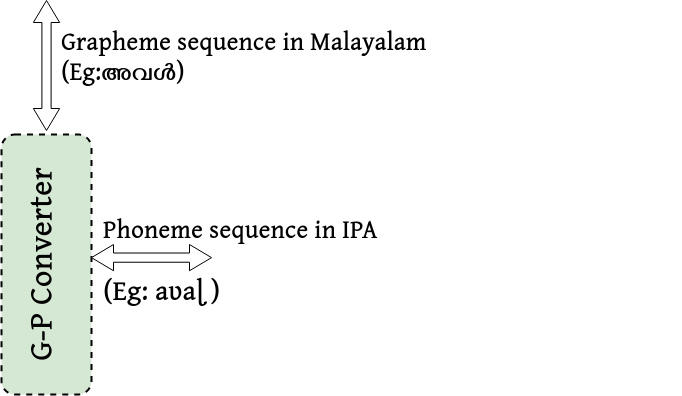
\includegraphics[scale=0.5]{g-pconverter-drawio.png}
	\caption{G-P Converter FST, performing phoneme analysis on the word {\mal അവൾ}.}
	% \Description{State Transition diagram of FST for phoneme analysis}
	\label{gpconverterfst}
\end{figure}

This FST, parses the words {\mal അവൾ}  {\ipa /aʋaɭ/}and {\mal അവൻ}  {\ipa /aʋan}/ in analysis mode as shown
in the Fig. \ref{g2pfst} (i). When operated in generate mode, it converts a
valid phoneme sequence into graphemes. For example, in generate mode, it can
parse the inputs {\ipa aʋaɭ} and {\ipa aʋan} as shown in Fig. \ref{g2pfst}
(ii).

\begin{figure}[htpb]
	\centering
	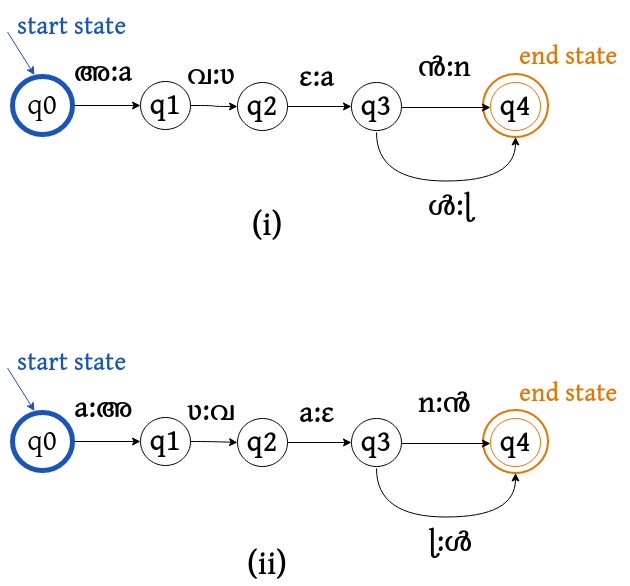
\includegraphics[width=0.6\linewidth]{g2p-fst-drawio.png}
	\caption{G2P converter FST performing (i) grapheme to phoneme conversion on the words  {\mal അവൾ} and {\mal അവൻ} in analysis mode and (ii) phoneme to grapheme conversion on {\ipa aʋaɭ} and {\ipa aʋan} in generate mode. }
	% \Description{State Transition diagram of FST for g2p}
	\label{g2pfst}
\end{figure}

% \begin{figure}[h]
% 	\centering
% 	\includegraphics[width=0.7\linewidth]{p2g-fst-drawio.png}
% 	\caption{G-P FST, performing phoneme to grapheme conversion on {\ipa aʋaɭ} and {\ipa aʋan} in generate mode }
% 	% \Description{State Transition diagram of FST for p2g}
% 	\label{p2gfst}
% \end{figure}
% The python script utilizing Mlphon library to perform grapheme to phoneme and the reverse operations are illustrated in Listings \ref{g2ppython} and \ref{p2gpython}.

\section{The Python Library: Mlphon}
\label{pypi}
The core functionalities of Mlphon is written in \gls{sfst} and compiled into different finite state transducers. SFST compiles the rules to form minimised FSTs which are very much memory optimised \cite{mohri-1997-finite}. The python binding of SFST provides access to these transducers for high level programming. Mlphon Python library is very compact with 21 kB of total file size.

One of the major motivation behind this work is to provide pronunciation
lexicon for integrating with ASR and TTS applications. The pronunciation
lexicon may require the transcriptions to have delimiters between phonemes
and/or syllables depending on the application. The utility functions
\texttt{split\_as\_phonemes} and \texttt{split\_as\_syllables} provided with
Mlphon python library can parse the phonemic analysis to a sequence of phonemes
or sequence of syllables separated by spaces. Additionally the function
\texttt{phonemise} accepts the delimiters defined by the user to separate
phonemes and syllables.

The Mlphon library also provides a command line utility for the tasks of
syllabification, phoneme analysis and conversion between graphemes and
phonemes. See Listing \ref{cli} for its usage and the list of optional
arguments. The entire development process was guided by a set of unit tests to
ensure expected functionalities.

\begin{lstlisting}[frame=tb,
	caption= Command line utility for Mlphon library,
	label={cli},
	basicstyle=\ttfamily\footnotesize
	]
mlphon [-h] [-s] [-a] [-p] [-pe string] [-se string] [-g] [-i INFILE]
        [-o OUTFILE] [-v]

optional arguments:
-h, --help            Show this help message and exit
-s, --syllablize      Syllablize the input Malayalam string
-a, --analyse         Phonetically analyse the input Malayalam string
-p, --tophoneme       Transcribe the input Malayalam grapheme to phoneme
                      sequence
-pe string, --phoneme_end string
                      String to be inserted at end of phoneme
-se string, --syllable_end string
                      String to be inserted at end of syllable
-g, --tographeme      Transcribe the input phoneme sequence to Malayalam
                      grapheme
-i INFILE, --input INFILE
                      Source of analysis data
-o OUTFILE, --output OUTFILE
                      Target of generated strings
-v, --verbose         Print verbosely while processing
\end{lstlisting}

\section{Intrinsic Evaluation of Mlphon}
\label{goldlexicon}

Evaluating a script analysis toolkit like Mlphon is not straight forward due
the absence of any baseline ground truth linguistic resource. A gold standard
manually annotated data, which can serve as a reference is an important
part of any quantifiable evaluation \cite{kayabacs2019trmor}. A gold standard
for \gls{g2p} conversion contains a list of words annotated with their true phoneme
transcription. A gold standard for syllabifier is annotated as a sequence of
syllables. If a word has multiple possible annotations, all of those should be
present in the gold standard lexicon. Before we explain the evaluation, the
following section presents the design of gold standard lexicon. It follows a
similar procedure and the number of entries as in \cite{kayabacs2019trmor},
used for creating a gold standard annotations for Turkish morphological
analyser.

\subsection{Design of Gold Standard Lexicon}

The lexical entries in gold standard lexicon are chosen from the IndicNLP
Corpus\footnote{\url{https://github.com/AI4Bharat/indicnlp_corpus}}
\cite{kunchukuttan2020ai4bharat} which is a list of words with frequency
information. These words belong to a general domain, web crawled Malayalam text
corpus of 167.4 million tokens with 8.8 million types.

The manually verified gold standard annotations were created
semi-automatically. The process began with the syllabification of 1000 of the
most common words in this corpus using Mlphon. It gave back a list of words,
some of which had the proper syllabification and others of which had none at
all. A small portion of the words that couldn't be syllabified were incorrectly
spelled, which is typical of a corpus compiled from web crawls. Misspelt words
were manually corrected in the corpus and syllabified. All the syllabifications
performed by Mlphon were also manually verified and corrected by expert
linguists, if found to be wrong. For the remaining words, which could not be
syllabified, manual annotation was performed. Thus the gold standard lexicon
for syllabification was obtained.

The gold standard lexicon for \gls{g2p} mapping followed a similar procedure. Mlphon
was used to phoneme map the spelling corrected 1000 words. The returned results
were manually corrected for deletion, substitution and insertion errors. The
manual corrections were performed, following all the rules and descriptions in
the reference books \cite{asher1997,prabo2016}. The removal of word final schwa
(\textit{samvruthokaram}) in proper nouns was suggested in a consultation with
linguists. The final annotations on the gold standard lexicon were approved by
them.

\begin{figure}[htpb]
	\centering
	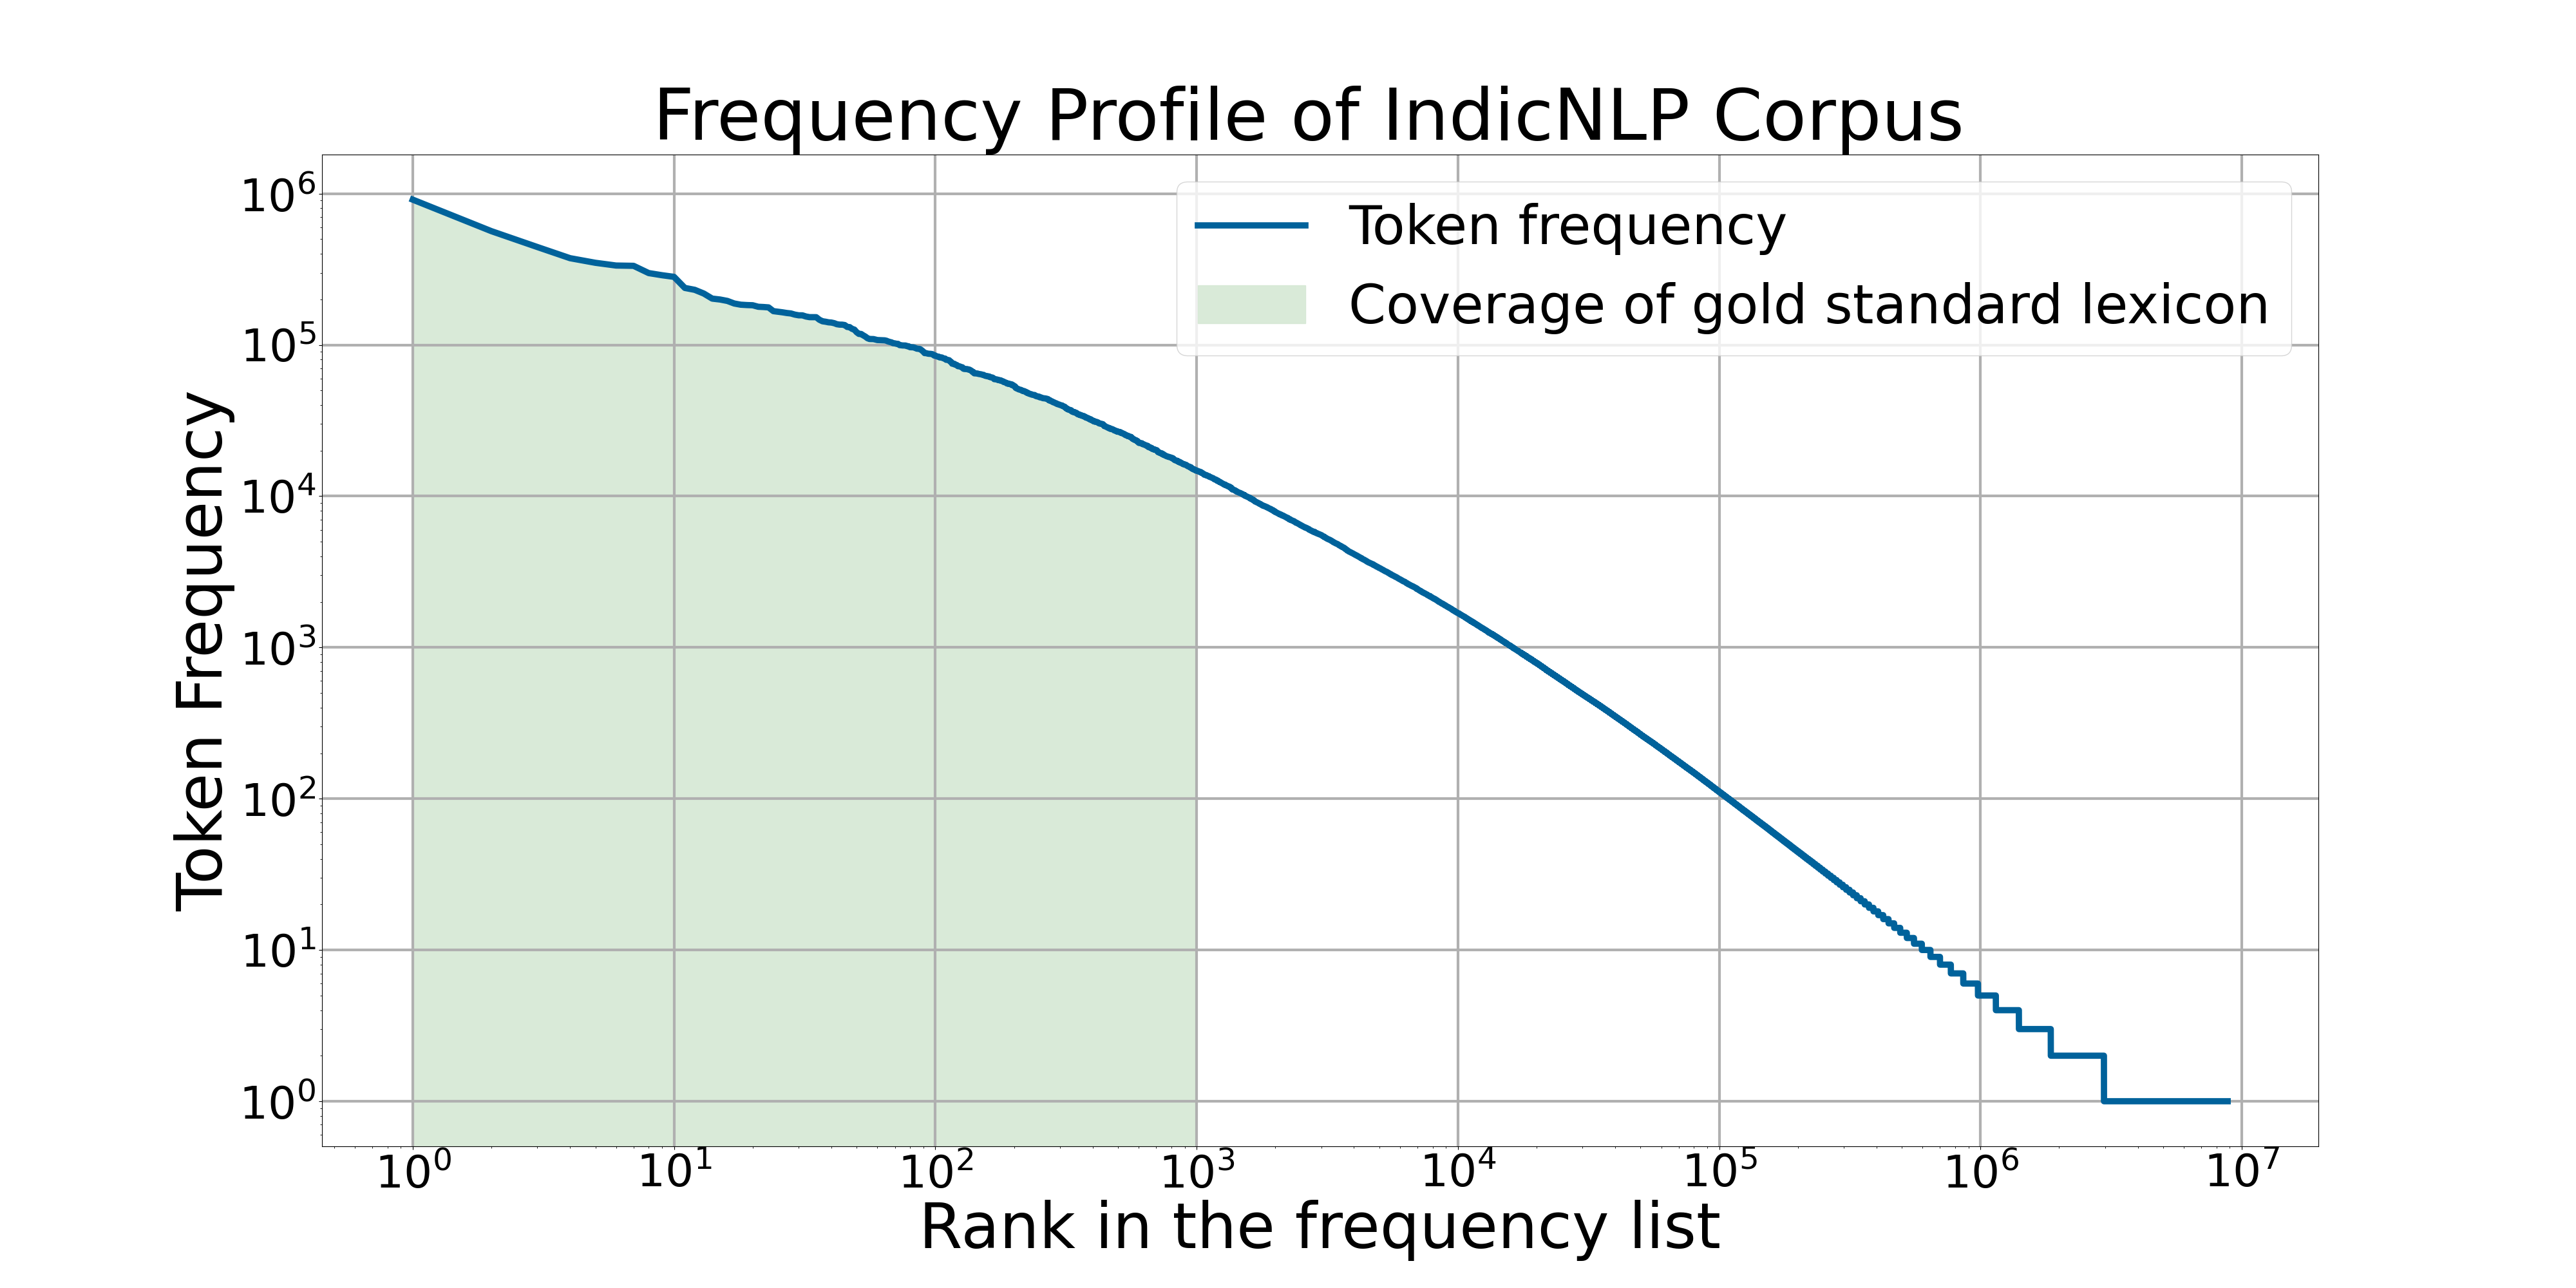
\includegraphics[width=0.8\linewidth]{rank.png}
	\caption{The lexical entries of gold standard lexicon is chosen from the most frequent thousand words from the IndicNLP corpus \cite{kunchukuttan2020ai4bharat} such that these words cover 26\% of the 167.4 million tokens present in this corpus.}
	\label{fig:rank}
	% Code Location: /home/kavya/researchdev/raw/
\end{figure}
\begin{figure}[htpb]
	\centering
	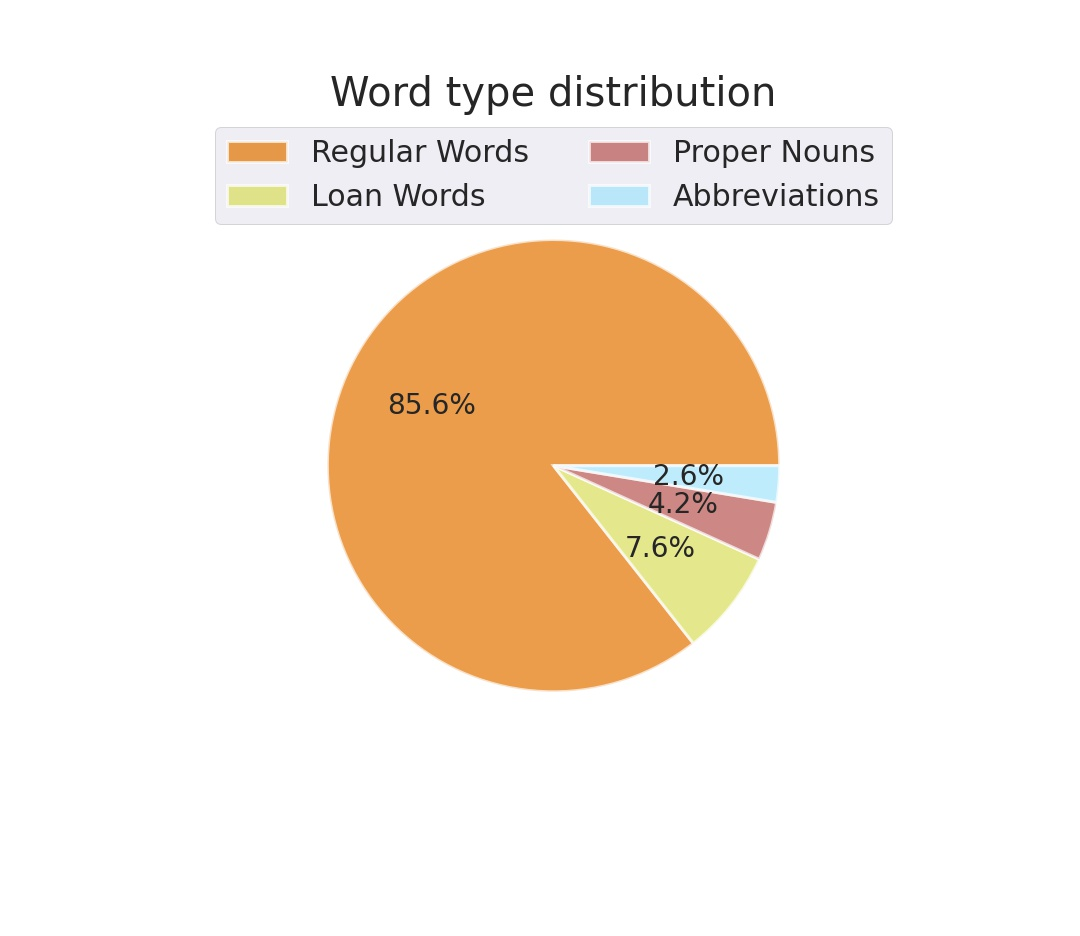
\includegraphics[trim={3cm 8cm 3cm 0cm},clip=true, width=0.8\linewidth]{wordtypes.jpg}
	\caption{Distribution of word types in gold standard lexicon}
	\label{fig:pie-chart}
	% Data Location: /home/kavya/tmp/phonemes/
\end{figure}

\begin{figure}[htpb]
	\centering
	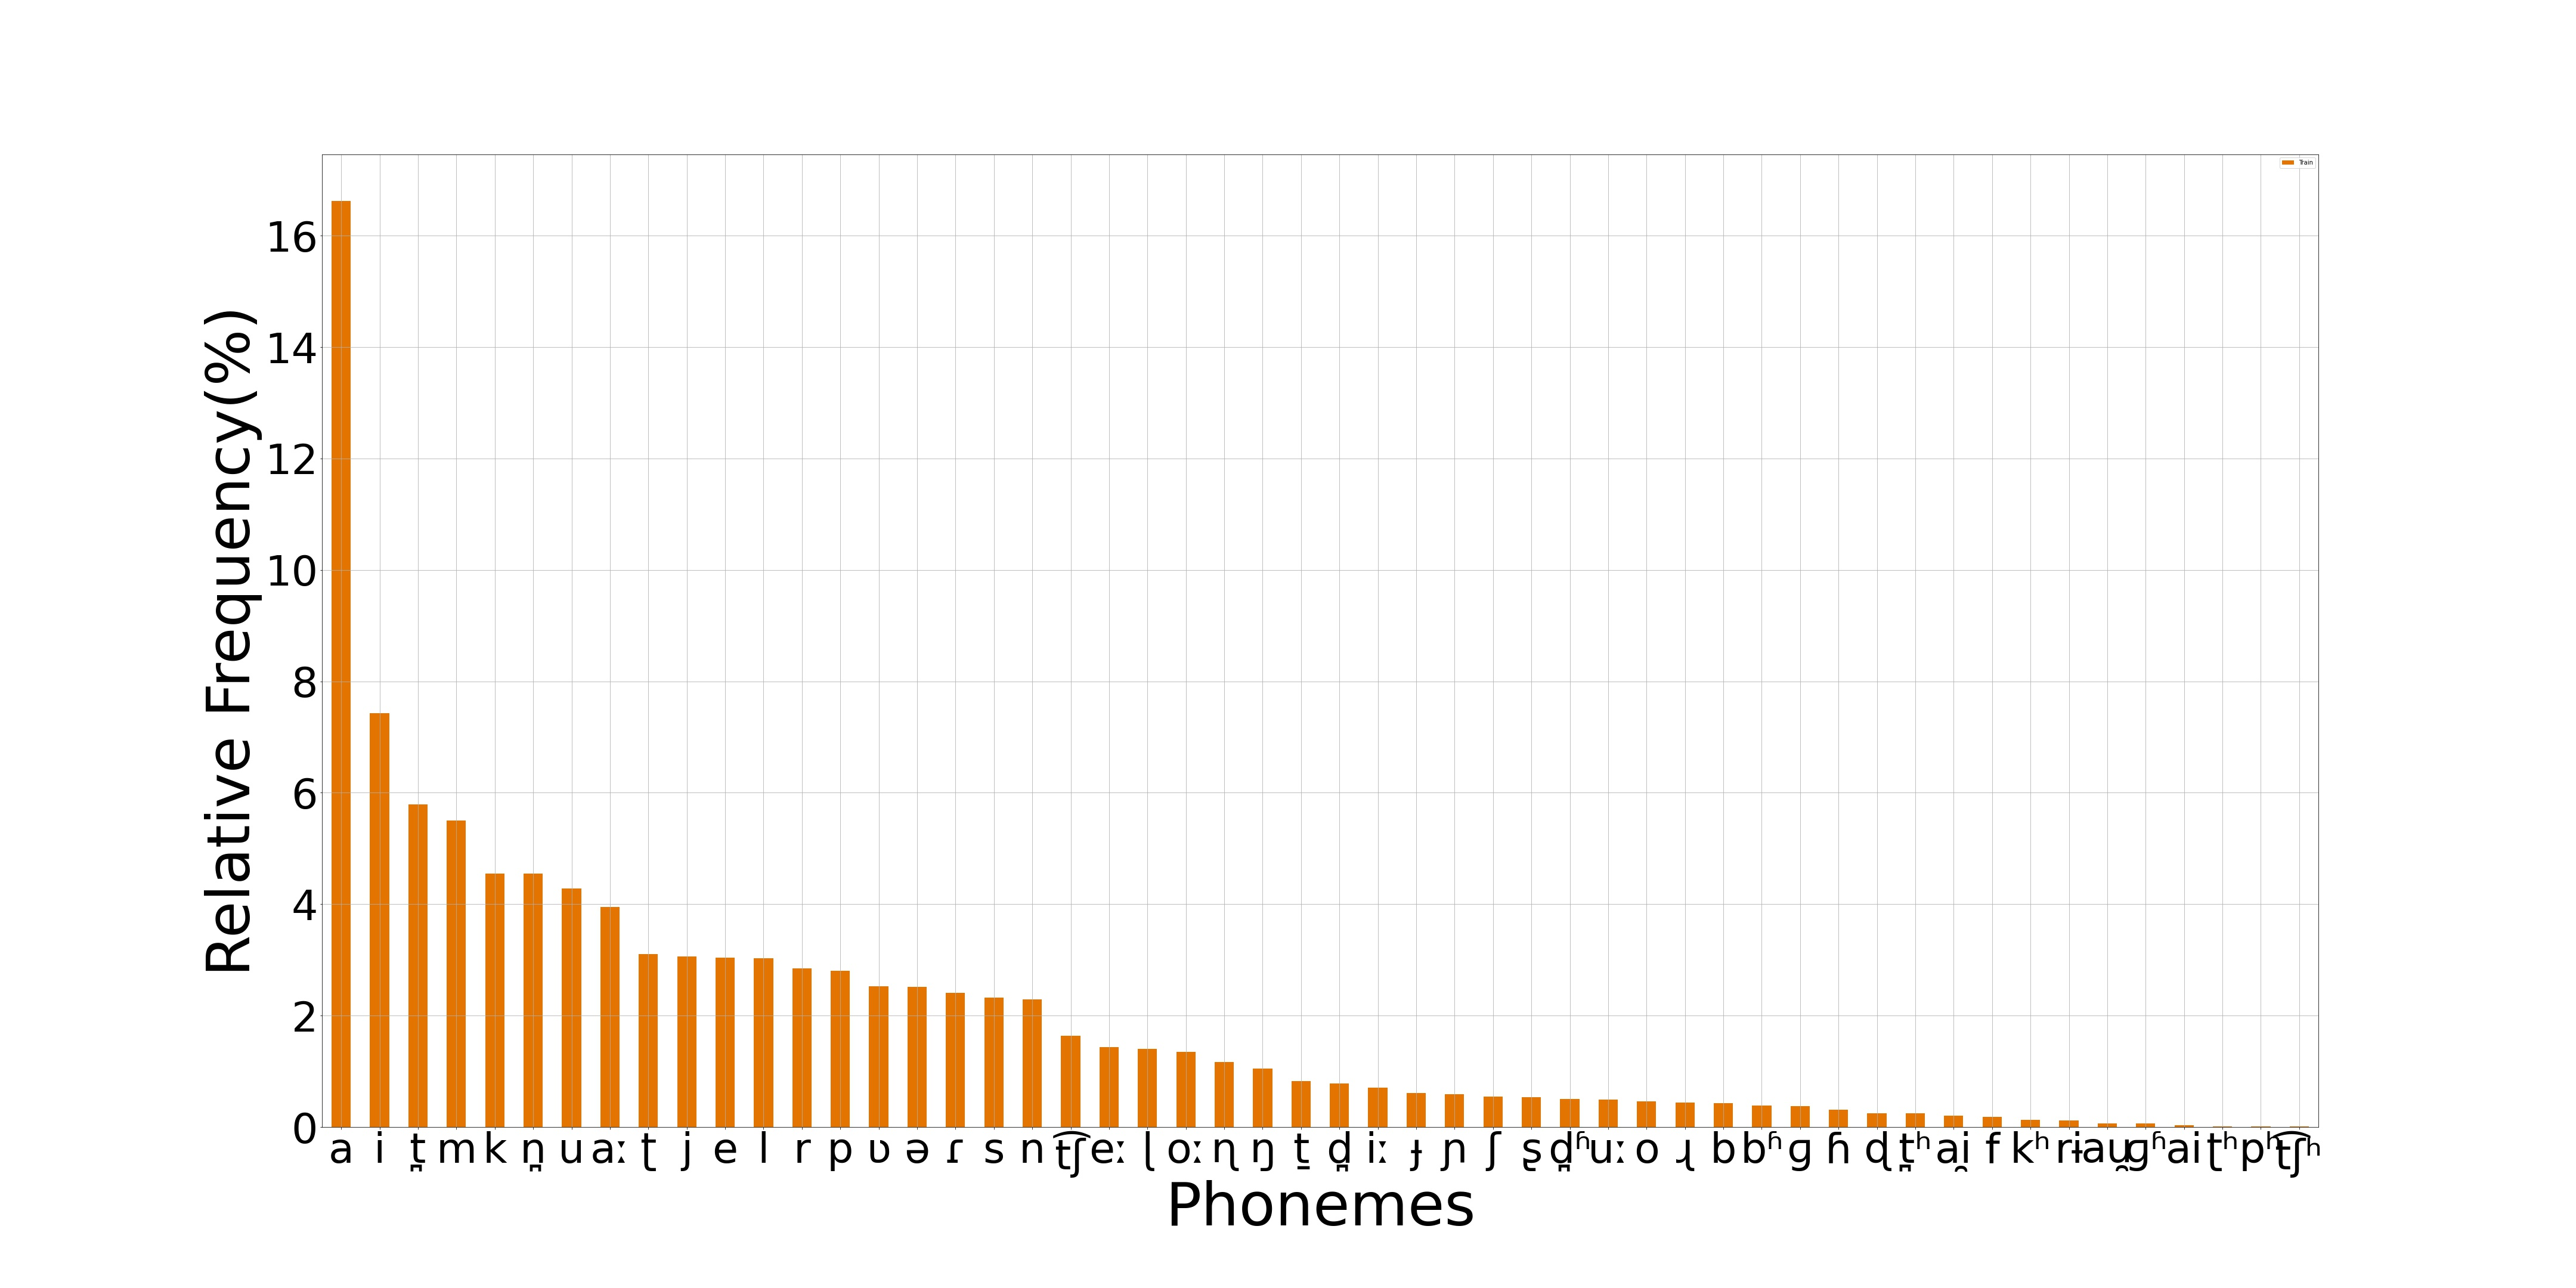
\includegraphics[width=\linewidth]{goldrichness.jpg}
	\caption{Phoneme diversity  analysis in gold standard lexicon}
	\label{fig:goldrichness}
\end{figure}

The lexical entries in the gold standard lexicon constitutes 26\% of the total
number of tokens in the said corpus according to the computation shown in
(\ref{eq:coverage-calc}). The frequency profile in Fig. \ref{fig:rank} illustrates
this. The coverage of tokens in the gold standard lexicon with respect to the
corpus is computed as:

\begin{equation}
	\label{eq:coverage-calc}
	\begin{split}
		Coverage & =\frac{\sum{}{}{Frequency\ of\ top\ 1000\ tokens} \times 100 }{Total\ token\ count\ in\ corpus}  \\ \\
		&  \approx \frac{44321494 \times 100}{167.4\ million} \\ \\
		& \approx 26 \%
	\end{split}
\end{equation}
The gold standard lexicon covers many regular words, loan words, proper nouns and abbreviations as per the distribution illustrated in Fig. \ref{fig:pie-chart}.



A phoneme diversity analysis of the gold standard lexicon was performed and
plotted in Fig. \ref{fig:goldrichness}. The relative frequency of phonemes in gold
standard lexicon follows the same pattern as previously reported values of
phoneme diversity in Malayalam speech corpora \cite{smcspeech}.

\subsection{Syllabification}

The syllabification results of Mlphon is evaluated on the gold standard
reference. Even though the syllabification rules are deterministic there has
been few deletion errors as illustrated in the Table \ref{tab:goldsyl} and analysed
in detail in section \ref{sec:Mlphon-errorsyl}.

\begin{table}[ht]
	\begin{center}
		% \begin{minipage}{\textwidth}
		\caption{Comparing the syllabification provided by Mlphon with gold standard \\reference.}
		\label{tab:goldsyl}
		\begin{center}
			\begin{tabular}{lllc}
				\hline \hline
				Word        & Reference      & Mlphon         & Error      \\ \hline
				{\mal ഈ}    & {\mal ഈ.}      & {\mal ഈ.}      & {-}        \\
				{\mal ഉന്നത} & {\mal ഉ.ന്ന.ത.} & {\mal ഉ.ന്ന.ത.} & {- }       \\
				{\mal എന്ന}  & {\mal എ.ന്ന.}   & {\mal എ.ന്ന.}   & {- }       \\
				{\mal  ഒരു}  & {\mal  ഒ.രു.}   & {\mal  ഒ.രു.}   & -          \\
				{\mal കഫേ}   & {\mal ക.ഫേ.}    & {\mal ക.ഫേ.}    & -          \\
				{\mal തോമസ്}  & {\mal തോ.മ.സ്.}  & {\mal തോ.മ.സ്.}  & -          \\
				{\mal നമ്പർ} & {\mal ന.മ്പർ.}  & {\mal ന.മ്പർ.}  & -          \\
				{\mal ഫലം}   & {\mal ഫ.ലം.}    & {\mal ഫ.ലം.}    & -          \\
				{\mal ഫോട്ടോ}  & {\mal ഫോ.ട്ടോ.}   & {\mal ഫോ.ട്ടോ.}   & -          \\
				% 			10 {\mal മുന്നറിയിപ്പ്} & {\ipa m u \textbf{n n} a r i j i p p ə} & m u {\ipa n̪ n̪} a r i j i p p ə} & Substitution \\

				{\mal സിഐഡി}  & {\mal സി.ഐ.ഡി. } & {\mal }        & {Deletion} \\ \hline
			\end{tabular}
		\end{center}

		% \end{minipage}
	\end{center}
\end{table}

\subsubsection{Syllabification Accuracy}

Accuracy is defined as a ratio between the correctly classified samples to the
total number of samples. Precision represents the proportion of positive
samples that were correctly classified to the total number of positive
predicted samples. Recall of a classifier represents the positive correctly
classified samples to the total number of positive samples. The harmonic mean
of precision and recall is the F1 score \cite{tharwat2020classification}. The
evaluation metrics averaged over all syllables and represented as percentage
has the values as listed here.
% \begin{equation}
% \label{accuracy}
% Accuracy = \frac{ (True\ Positives + True\ Negatives) }{Total\ Samples}
% \end{equation}
%  as indicated in (\ref{pre}).
% \begin{equation}
% \label{pre}
% Precision = \frac{ True\ Positives }{(True\ Positives + False\ Positives)}
% \end{equation}

% \begin{equation}
% \label{recall}
% Recall = \frac{ True\ Positives }{(True\ Positives + False\ Negatives)}
% \end{equation} \cite{tharwat2020classification} as indicated in (\ref{f1}).
% \begin{equation}
% \label{f1}
% F1\ Score = \frac{(2 * Precision * Recall)} {(Precision + Recall)}
% \end{equation}

\begin{lstlisting}[basicstyle=\ttfamily]
	Accuracy	: 99%
	Precision	: 99%
	Recall		: 99%
	F1 Score	: 99%
\end{lstlisting}

\subsubsection{Syllable Error Rate}

We measure the syllable error rate (SER) based on the number of insertions,
deletions, and substitutions for every syllable present in the gold standard
lexicon.
% The result is given below.

% \begin{equation}
% 	\label{SER}
% 	SER = \frac{(I+D+S) × 100}{(N)}
% \end{equation}

\begin{lstlisting}[basicstyle=\ttfamily]
	Total Words: 1000
	Total Syllables:  2891
	Syllables deleted: 18
	Syllables Inserted: 0
	Syllables Substituted: 0
	Syllables Error Rate: 0.62%
\end{lstlisting}

\subsubsection{Syllable Error Analysis on Different Word Types}
\label{sec:Mlphon-errorsyl}

Among the words in gold standard lexicon, all syllabification errors were
concentrated in words that are English abbreviations directly transliterated to
Malayalam without any delimiters in between. Such words have violated the
script grammar of Malayalam with vowels in word medial positions. Some Arabic
loan words are among the other valid words that defy script grammar and cannot
be syllabified by Mlphon.

\begin{figure}[ht]
	\centering
	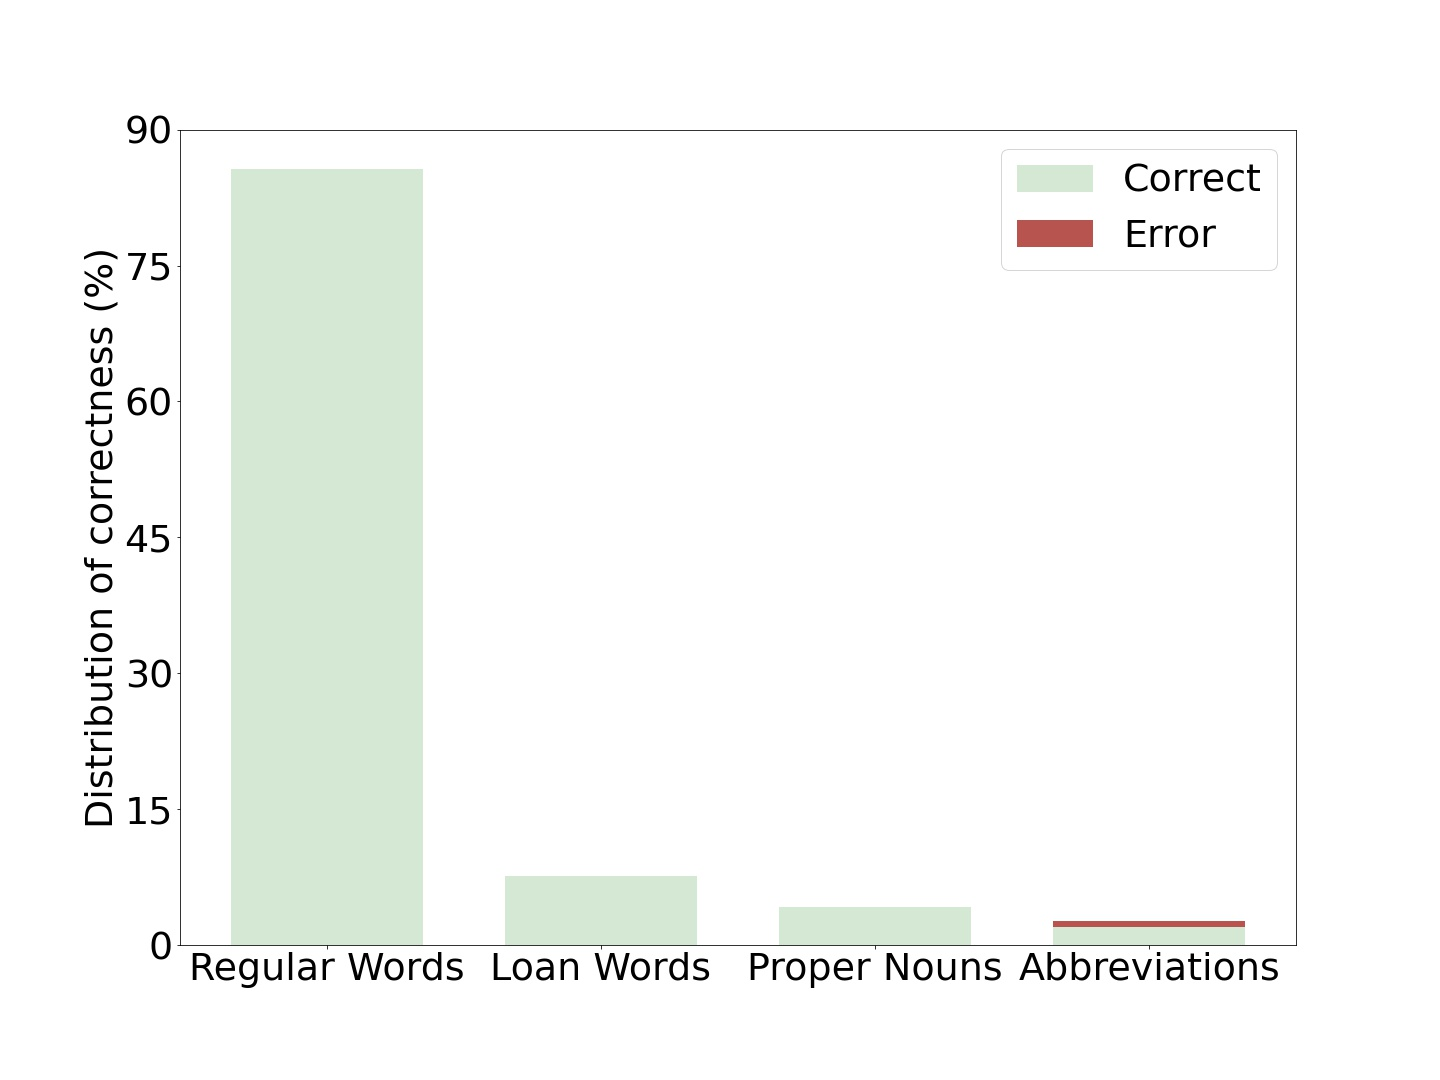
\includegraphics[width=0.8\linewidth]{syllable-error.jpg}
	\caption{Distribution of syllabification errors in different word types in gold standard lexicon}
	\label{fig:syllable-error}
\end{figure}

When the word level syllabification errors were examined, 23\% of the
abbreviations were incorrectly syllabified. This makes up about 0.6\% of words
in the entire gold standard lexicon. It is illustrated in Fig.
\ref{fig:syllable-error}.

\subsection{Grapheme to Phoneme Conversion}

% As per the observations in 

% Word medial vowel graphemes which are considered to be invalid  by Mlphon, leads to deletion of that word without syllabification. However these errors could be corrected automatically by splitting the  words at positions of word medial vowels and passing as tokens to Mlphon. The following analysis on g2p conversion has been done after performing this correction.

The \gls{g2p} conversion of Mlphon is evaluated, comparing its output
with gold standard phoneme transcriptions. Evaluation involves phoneme level
alignment of the transcription provided by Mlphon with that of the gold
standard lexicon and counting the number of insertions, deletions and
substitutions. We use the toolkit Kaldialign\footnote{Kaldialign library
	\url{https://pypi.org/project/kaldialign/}} to perform the same. A sample of
gold standard transcriptions with the phoneme sequence output provided by
Mlphon is shown in Table \ref{tab:gold}.
% As discussed in section \ref{syllabletagger}, Mlphon checks for validity of character sequences. If there are vowel graphemes at middle of words, it is flagged as a lingustically invalid sequence and not parsed by FST. It is a common paractice in everyday news articles to have English acronyms transliterated to Malayalam without any delimiters (periods or spaces) in between. It effectively acts as a single word which has vowel graphemes at word middle positions. Such acronyms which are not transcribed by Mlphon, leads to deletion errors. In order to transcribe those acronyms, they are split at the positions of word medial vowels and are passed as tokens to Mlphon library. This is how the eleventh entry {\mal സിഐഡി} (C.I.D), with the vowel {\mal ഐ} in word medial position is correctly transcribed in the Table \ref{gold}.

\begin{table}[htpb]
	\begin{center}
		% \begin{minipage}{\textwidth}
		\caption{Comparing the G2P transcription provided by  Mlphon with gold standard reference.}
		\label{tab:gold}
		\begin{tabular}{llll}
			\hline\hline
			Word        & Reference                   & Mlphon                                & Error        \\
			\hline
			{\mal ഈ}    & {\ipa iː}                   & {\ipa iː}                             & -            \\
			{\mal ഉന്നത} & {\ipa u n n a t̪ a}          & {\ipa u n n a t̪ a}                    & -            \\
			{\mal  എന്ന} & {\ipa e n̪ n̪ a }             & {\ipa e n̪ n̪ a}                        & -            \\
			{\mal  ഒരു}  & {\ipa o ɾ u }               & {\ipa o ɾ u}                          & -            \\
			{\mal കഫേ}   & {\ipa k a f eː}             & {\ipa k a f eː}                       & -            \\
			{\mal തോമസ്}  & {\ipa t̪ oː m a s}           & {\ipa t̪ oː m a s} \textbf{{\ipa  ə}}  & Insertion    \\
			{\mal നമ്പർ} & {\ipa \textbf{n} a m p a r} & \textbf{{\ipa n̪  }} {\ipa  a m p a r} & Substitution \\
			{\mal ഫലം}   & {\ipa  pʰ a l a m}          & {\ipa pʰ a l a m}                     & -            \\
			{\mal ഫോട്ടോ}  & {\ipa f oː ʈ ʈ oː}          & {\ipa f oː ʈ ʈ oː}                    & -            \\
			% 			10 {\mal മുന്നറിയിപ്പ്} & {\ipa m u \textbf{n n} a r i j i p p ə} & m u {\ipa n̪ n̪} a r i j i p p ə} & Substitution \\
			{\mal സിഐഡി}  & {\ipa s i ai̯ ɖ i }          & {\ipa s i ai̯ ɖ i }                    & -            \\
			\hline
		\end{tabular}
		% \end{minipage}
	\end{center}
\end{table}

\subsubsection{G2P Conversion Accuracy}

Comparing the true phonemes in gold standard lexicons to the transcription
provided by Mlphon, we present the phoneme transcription accuracy in the form
of a confusion matrix in Fig. \ref{fig:confusionmatrix}. For all phonemes other
than those listed in Table \ref{tab:precision}, the accuracy, precision, recall,
and F1 scores were computed to be 100\%. \vspace{0.2cm}

\begin{table}[htpb]
	\begin{center}
		% 		\begin{minipage}{190pt}
		\caption{Precision, Recall and F1 Scores of phoneme transcription by Mlphon. For all other phonemes, these metrics are evaluated to be 100\%.}
		\label{tab:precision}
		\begin{tabular}{@{}cccc@{}}
			\hline\hline
			Phoneme  & Precision (\%) & Recall (\%) & F1 Score (\%) \\
			\hline
			{\ipa n} & 100            & 84          & 91            \\
			{\ipa n̪} & 92             & 100         & 96            \\
			{\ipa ə} & 93             & 100         & 97            \\

			\hline
		\end{tabular}
		% 		\end{minipage}
	\end{center}
\end{table}

Except for the {\mal ന} disambiguation rules, all contextual rule sets operate
flawlessly without a single error when evaluated on gold standard lexicon. The
unintentional insertion of \textit{samvruthokaram} into non native proper names
and abbreviations transliterated from English was the cause of all the
insertion errors. Insertion is mapped to the empty symbol `\#' in the gold
standard transcription. The top row of the Fig.\ref{fig:confusionmatrix} shows
insertion of `{\ipa ə}'. Since the mostly ambiguous grapheme {\mal ഫ} was \gls{g2p}
mapped with 100\% accuracy on the gold standard lexicon, we increased the
evaluation space to include 100k common Malayalam words. According to the
confusion matrix in Fig. \ref{fig:faconfusion}, the transcription accuracy of {\mal
		ഫ} dropped to 99\% in the expanded evaluation set.

% There are some ambiguities in resolving alveolar nasal from dental nasal as listed in rows 7 of Table \ref{gold} and it can be clearly seen in the confusion matrix too.However there has been no occurrence of wrong mapping of the {\mal ഫ} in the  gold standard lexicon.

The overall evaluation metrics averaged over all phonemes in the gold standard
lexicon has the values in percentage as listed here.

\begin{lstlisting}[basicstyle=\ttfamily]
	Accuracy	: 99%
	Precision	: 98%
	Recall		: 98%
	F1 Score	: 98%
\end{lstlisting}

\begin{figure}[htpb]
	\centering
	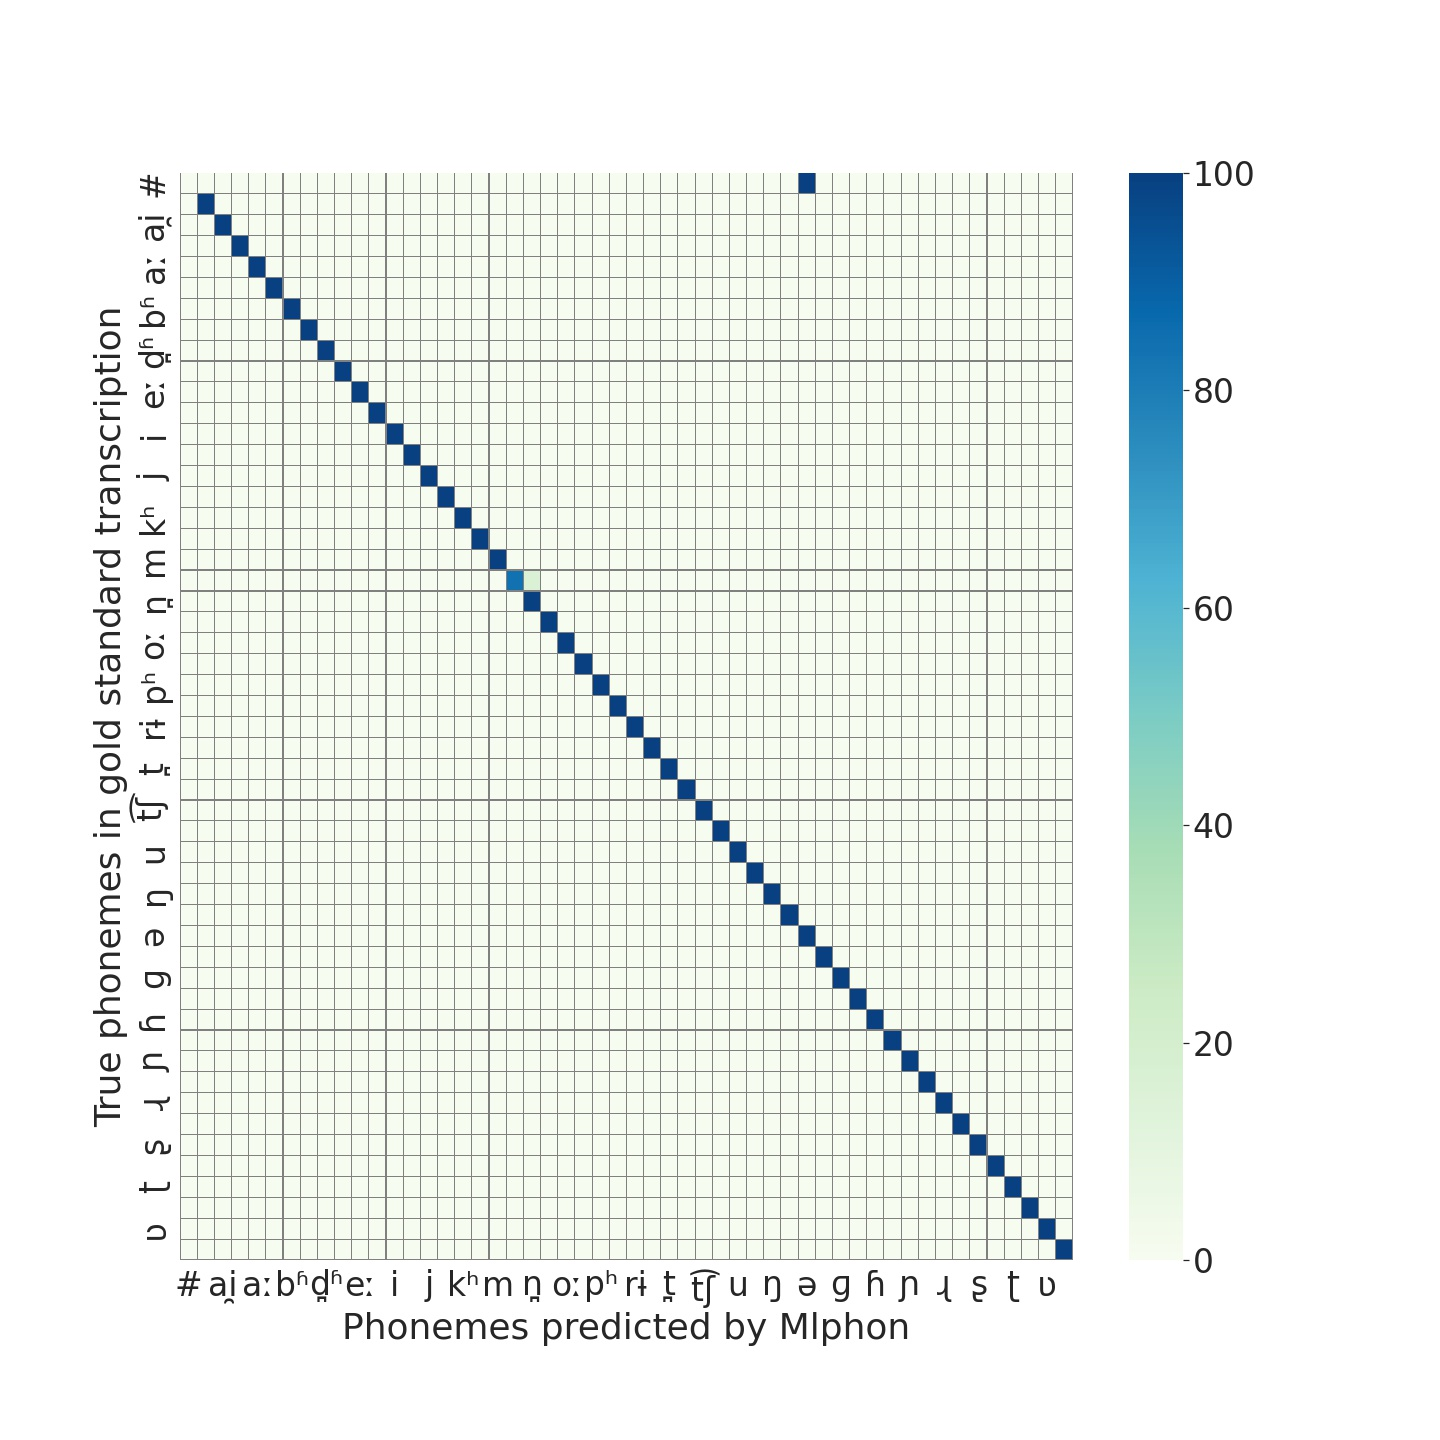
\includegraphics [width=0.9\linewidth]{confusion.jpg}
	\caption{Confusion matrix comparing Mlphon transcription with gold standard transcription. The values are normalised and represented as percentage.}
	% \Description{Confusion matrix comparing Mlphon transcription with gold standard transcription}
	\label{fig:confusionmatrix}
\end{figure}

\begin{figure}[!ht]
	\centering
	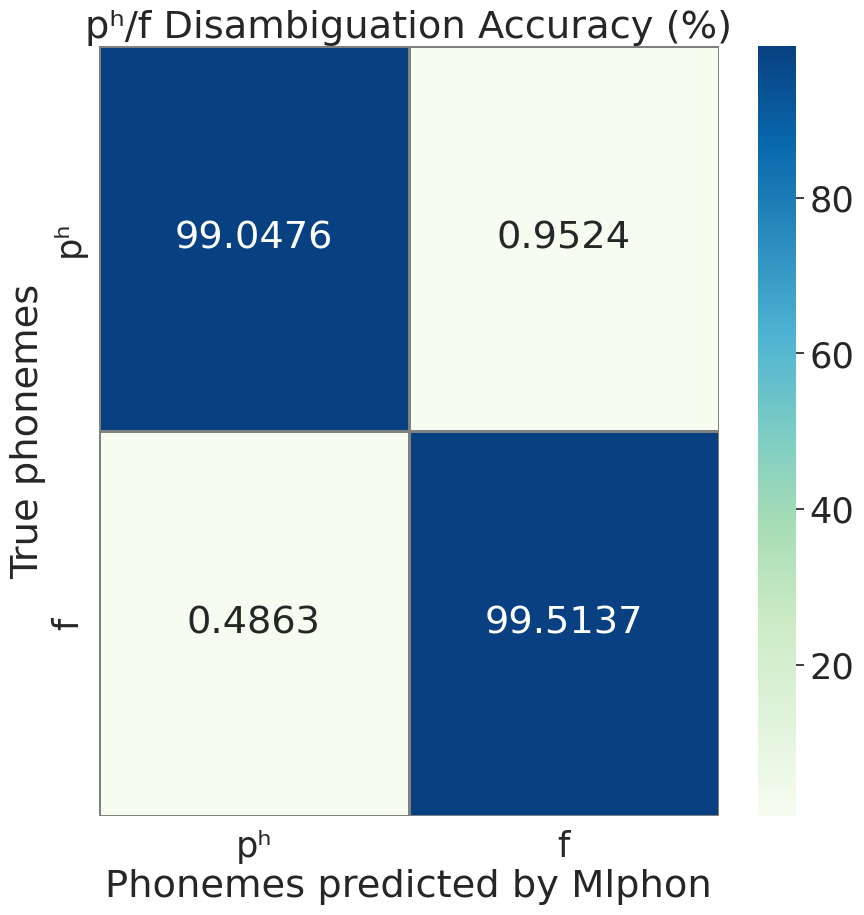
\includegraphics[width=0.6\linewidth]{fa.png}
	\caption{In an evaluation space of 100k tokens, we computed the accuracy of transcribing  {\mal ഫ}. The two possible pronunciations /{\ipa f}/ and /{\ipa pʰ}/ were accurately identified in more than 99\% of the cases as shown in this confusion matrix.}

	% Confusion matrix comparing transcription errors of  in a lexicon of 100k common words. The values are normalized and represented as percentage.}
	% \Description{Confusion matrix comparing transcription errors of {\mal ഫ} in a lexicon of 100k common words.}
	\label{fig:faconfusion}
\end{figure}

\subsubsection{Phoneme Error Rate}

As an alternate metric to measure the phoneme transcription quality, we
evaluate the \gls{per}. It is computed based on the number of
insertions, deletions, and substitutions for every phoneme present in the gold
standard lexicon.

% \begin{equation}
% 	\label{PER}
% 	PER = \frac{(I+D+S) × 100}{(N)}
% \end{equation}

\begin{lstlisting}[basicstyle=\ttfamily]
	Total Words: 1000
	Total Phonemes:  6755
	Phonemes deleted: 0
	Phonemes Inserted: 12
	Phonemes Substituted: 25
	Phoneme Error Rate = 0.55%
\end{lstlisting}

\subsubsection{G2P Error Analysis on Different Word Types}

We performed a detailed analysis of \gls{g2p} errors on different types of words in
the gold standard lexicon. 1.4\% of regular words and 1.3\% of loan words had
substitution errors. About 23\% of proper nouns and 15\% of abbreviations had
insertion errors due to unintended \textit{samvruthokaram} at word ends. All
the erroneous words account for 2.6\% of the total words in the gold standard
lexicon. It is illustrated in Fig. \ref{fig:g2p-error}.

\begin{figure}[ht]
	\centering
	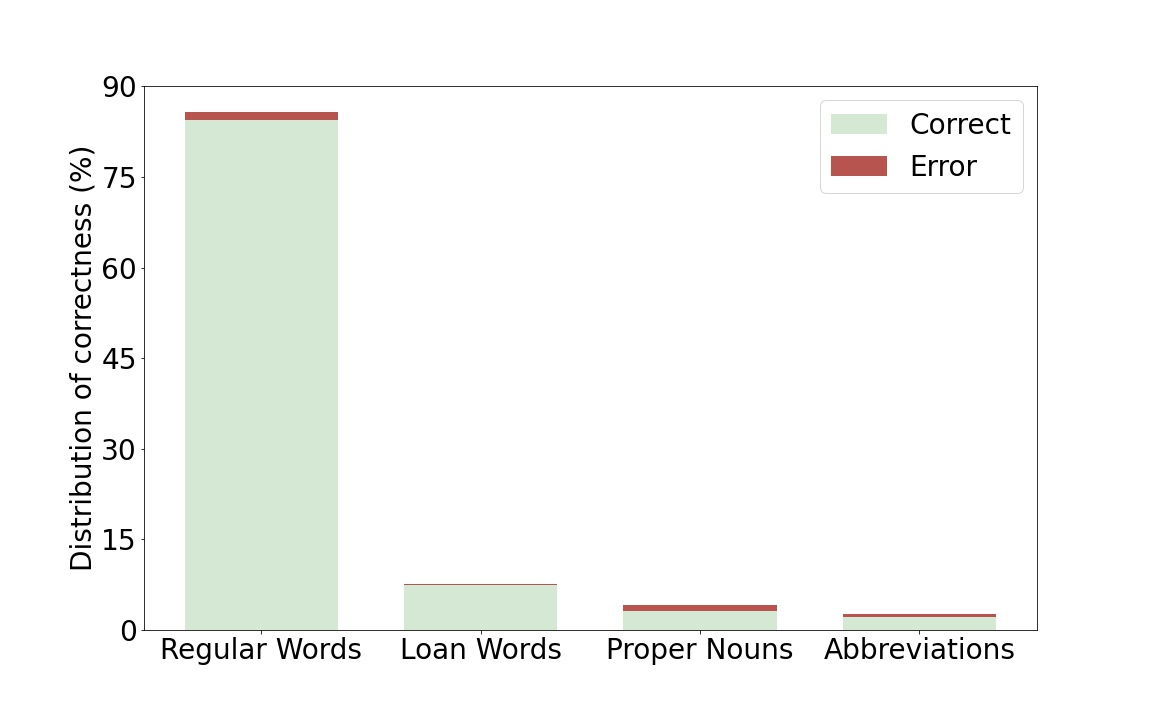
\includegraphics[width=0.8\linewidth]{g2p-error.jpg}
	\caption{Distribution of G2P errors in different word types in gold standard lexicon.}
	\label{fig:g2p-error}
\end{figure}

% All the contextual rule sets work perfectly without errors except the disambiguation rules for {\mal ന}. All the insertion errors are due to unintended insertion of \textit{Samvruthokaram} in non-native proper names. Since {\mal ഫ} is transcribed in the gold standard lexicon with 100\% accuracy, we expanded the evaluation space to 100k common words in Malayalam. It gave an accuracy above 99\% for transcription of {\mal ഫ} as shown in the confusion matrix in Fig. \ref{faconfusion}.

The correction of substitution and insertion errors involve morphologically
analysing the words, which is currently beyond the scope of this work. Even
with these limitations, the PER on the gold standard lexicon that covers about
26\% of words from 167 million tokens is only 0.55\%
% \section{DISCUSSION WITH OTHER TOOLS ON G2P TASK}

% The pronunciation lexicon contains words and their pronunciation as a sequence of phonemes.

% To create a pronunciation lexicon for training the ASR, we have chosen the 100k common words lexicon described in Section \ref{pronunciationdictionary}. It is then expanded with the words from the training audio transcripts and words with atleast four occurrences from the language model training corpus. 

%We employ the pipeline approach for ASR architecture where the the acoustic model, the pronunciation lexicon and the language model are different components that work together as a system. 

%
% In the pipeline approach, transcribed audio data requirement is much lesser than that in an end-to-end architecture of ASR for the same level of recognition accuracy \cite{Rosenberg2017, drexler2020improving}. This factor is very crucial considering the low resource nature of Malayalam.

%Many end-to-end systems are prohibitive to be used in embedded system applications due to their high computational and memory requirements. Kaldi TDNN chain model has proven to be an optimal solution with minimum memory and computational requirements for use in embedded applications without much compromising the recognition accuracy \cite{georgescu2021performance}.  To ensure good performance on embedded applications as well, we use Kaldi toolkit \cite{povey2011kaldi} for our experiments on ASR, with pronunciation lexicons created using Mlphon .

%(ii) Phonemizer\footnote{Python package phonemizer \url{https://pypi.org/project/phonemizer/}}  with Espeak backend and (iii) Unified Parser\footnote{Unified Parser source code \url{https://www.iitm.ac.in/donlab/tts/unified.php}}  \cite{baby2016unified}.

%\subsubsection{Speech Datasets}

%We have employed publicly available Malayalam speech corpora present in different multilingual datasets, namely,

% The speech datasets used are OpenSLR\footnote{OpenSLR Malayalam speech corpus \url{http://openslr.org/resources/63/}} \cite{he-etal-2020-open}, Indic TTS \cite{baby2016resources} and Festvox IIITH database\footnote{Festvox IIITH Malayalam speech corpus \url{http://www.festvox.org/databases/iiit_voices/}} \cite{prahallad2012iiit}. The entire Indic TTS speech database is used for training, Festvox IIITH speech database is set aside for testing, Open SLR corpus is split into two parts, one for training and the other for testing.  We have strictly ensured there is no overlap of speakers in training and test datasets.

%\begin{table}
%	\caption{Training Speech corpora}
%	\label{trainingcorpus}
%	\begin{tabular}{cccc}
%		Corpus           & Duration   & Utterances & Speakers \\
%		& (HH:MM:SS) &            &          \\
%		\toprule
%		Open SLR (train) & 4:47:47    & 3446       & 37       \\
%		Indic TTS        & 13:58:20   & 8601       & 2        \\
%		\midrule
%		Total            & 18:46:07   & 12047      & 39       \\
%		\bottomrule
%	\end{tabular}
%\end{table}
%
%% \begin{table}
%% 	\caption{Test Speech corpora}
%% 	\label{testingcorpus}
%% 	\begin{tabular}{cccc}
%% 		Corpus & Duration  & Utterances & Speakers \\
%% 		 & (HH:MM:SS) & & \\
%% 		\toprule
%% 		Open SLR (test) &  00:48:02 & 680 & 5 \\
%% 		Festvox IIITH &  01:37:46 & 1000 & 1 \\
%% 		\bottomrule
%% 	\end{tabular}
%% \end{table}

%\subsubsection{Text Corpus for Language Modeling}

% Remaining 212k sentences are cleaned up to remove special characters, numerals and then they are unicode normalised to get the text corpus for language model training.
% The language model training corpus contain 212k unique sentences and 26k unique words.

% \subsubsection{Creation of Large Vocabulary Pronunciation Lexicon}
% \label{lexiconcreation}

% The pronunciation lexicon for ASR is created with this 121k words using Mlphon, which took 1 minute 45 seconds to complete 
% Mlphon is capable of automatic creation of pronunciation lexicon consuming considerably less amount of processing time. The reason for the time efficiency while using Mlphon can be attributed to the computationally fast determinised FSTs \cite{mohri-1997-finite}, upon which Mlphon is built.

\section{Applications of Mlphon}
\label{applications}
In this section we describe some potential application of Mlphon. The applications include  phonemic diversity analysis of speech corpora, assisted pronunciation learning, text sanity check and correction and creation of large vocabulary pronunciation lexicon. These are described in the following subsections.

% \subsection{Syllable based Language Modeling}

% The syllabification module in Mlphon is a standalone unit that splits words to syllables. It has been demonstrated in literature that subword based models are better in capturing language features for morphologically complex languages \cite{SMIT2021101158}. Syllables serve as a good choice of subwords for practical applications including automatic speech recognition \cite{adiga-etal-2021-automatic} that takes care of OOV scenarios. Orthographic syllable units have proven to be more effective in statistical machine translation, than other basic units (word, morpheme and character) when trained over small parallel corpora  \cite{kunchukuttan2016}. Mlphon can be employed in  various applications that require syllable level language modeling.

% As an example, we demonstrate the usage of syllable based lexicons and language models on ASR task. We use the same experimental setup as described in section \ref{asr}. Evaluation is done on OpenSLR test set where OOV is higher. To evaluate syllable based language models and lexicons, we use word based lexicons and language models as baseline. The Fig. \ref{subword}, shows how the WER of syllable  based lexicons and language models are consistently better than word based ones,  while incrementally increasing the vocabulary size. Each subword lexicon is built by including all the syllables present in corresponding word lexicon. For example the first subword lexicon has 3.5k syllables as entries, obtained by syllabifying every entry in corresponding word lexicon with 25k entries. It is observed that syllable based ASR performed much better than word based ones, as it recovered many OOV words by reconstructing words by concatenating syllables. 
% % However word based ones had better performance on test set T1, where the OOV rates were low (1\% OOV).

% \begin{figure}[h]

% 		\centering
% 		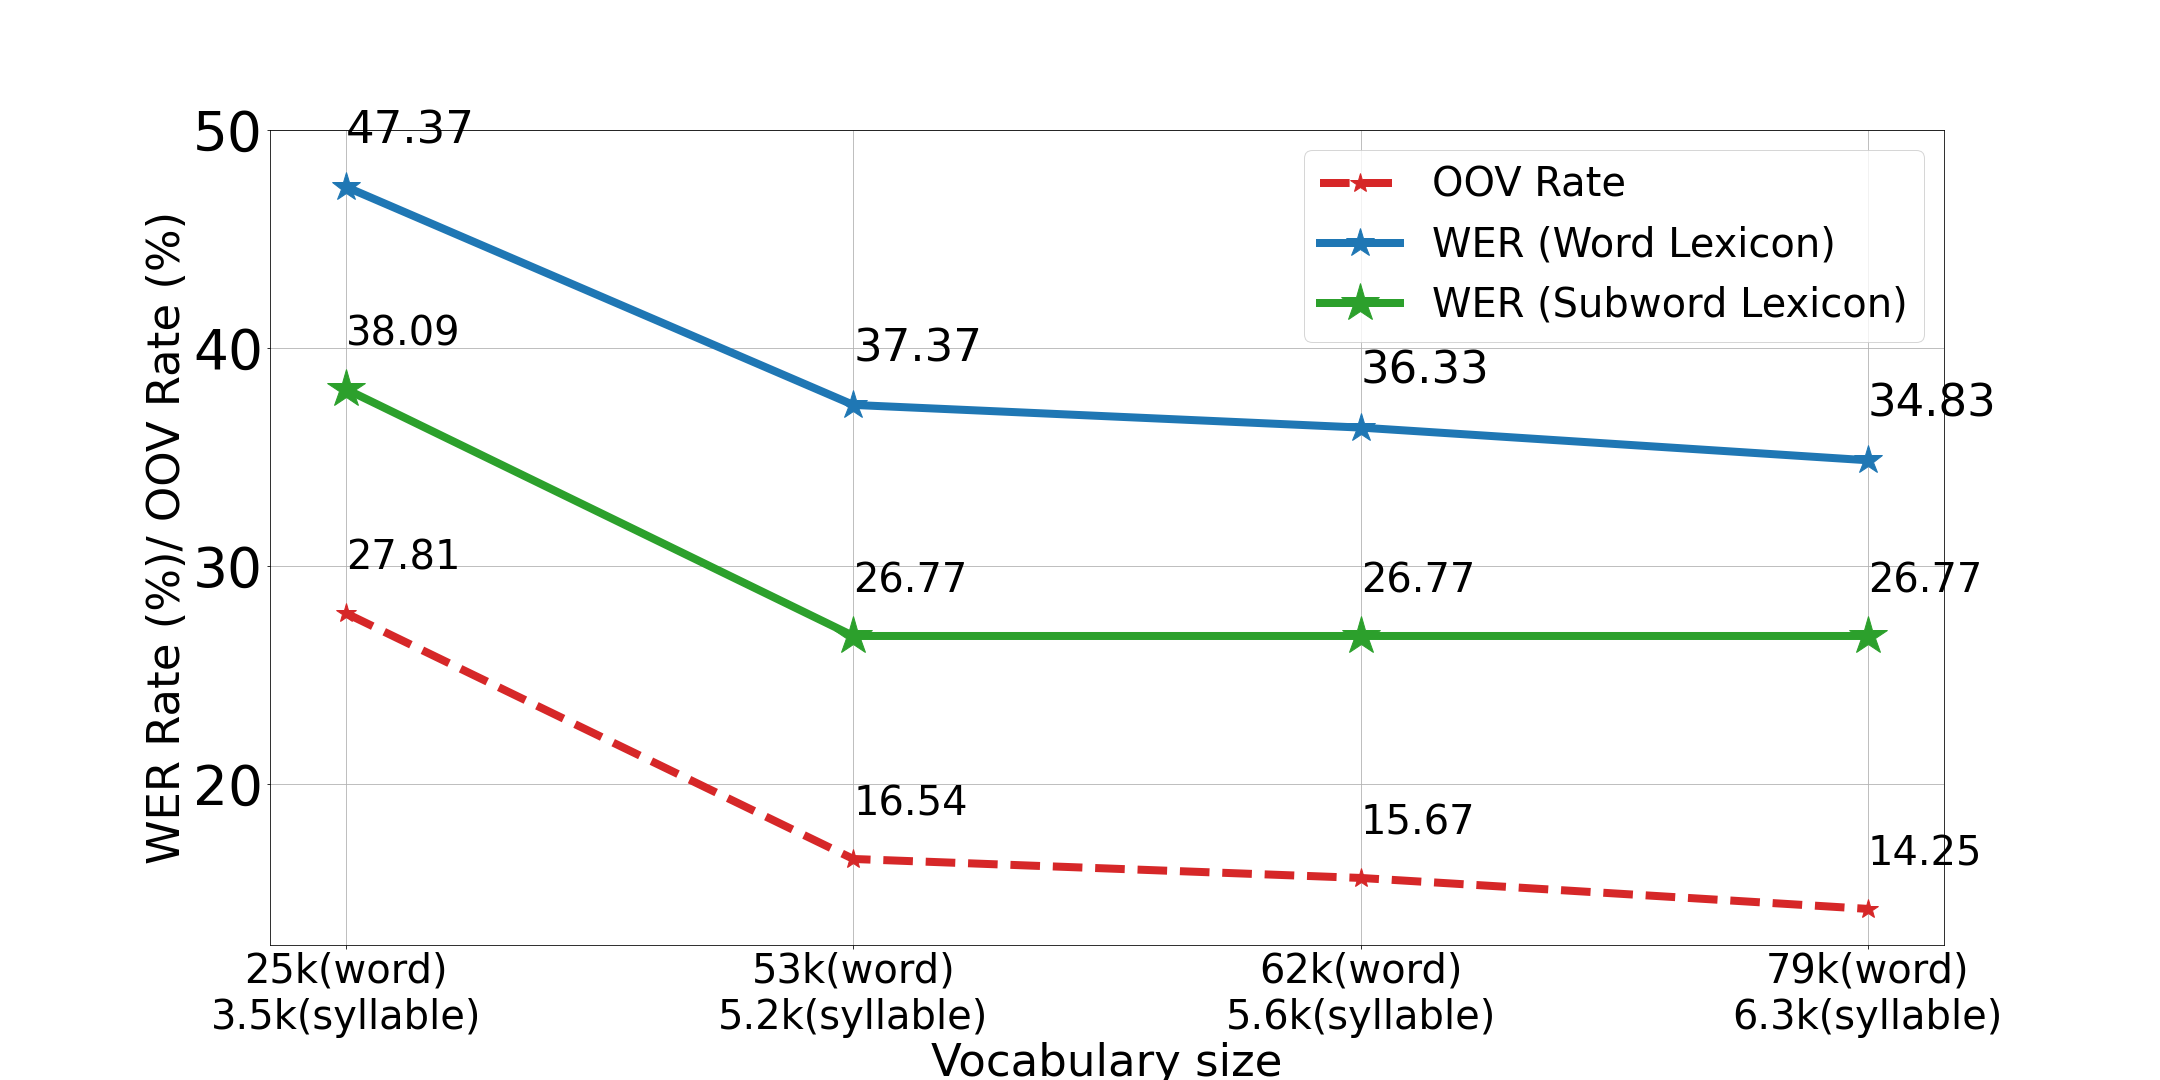
\includegraphics[width=\linewidth]{trigramT2.png}
% 	\caption{Plot showing WER obtained in Malayalam ASR experiments with word based and syllable subword based language models and lexicons. Word vocabulary sizes are indicated on x-axis.}
% 			\label{subword}
% %
% \end{figure}

\subsection{Phonemic Diversity Analysis of Speech Corpora}

Speech corpus used in developing ASR and TTS systems has to be phonemically
balanced and rich to ensure proper acoustic modelling
\cite{malviya2016structural}. We transcribed the speech corpus transcript to
phonemised text using Mlphon. The phoneme diversity of the resulting text is
then analysed. The graph in Fig. \ref{phoneticrichness} illustrates the
phonemic richness of the corpora used in the ASR experiments described in
chapter \ref{ch:lvcsr}. The phoneme with the highest number of appearances is the
inherent vowel {\ipa /a/}, followed by the vowel {\ipa /i/} in all the corpora
under consideration. The most frequent consonant phoneme is the dental plosive
	{\ipa /t̪/} in Indic TTS \cite{baby2016resources} corpus while it is {\ipa /n̪/}
in OpenSLR \cite{he-etal-2020-open} and Festvox IIITH \cite{prahallad2012iiit}
corpora. The statistical analysis of phonemes could potentially be used to
design corpora with phonemically balanced content \cite{torres2019emilia}.

\begin{figure}[htpb]
	\centering
	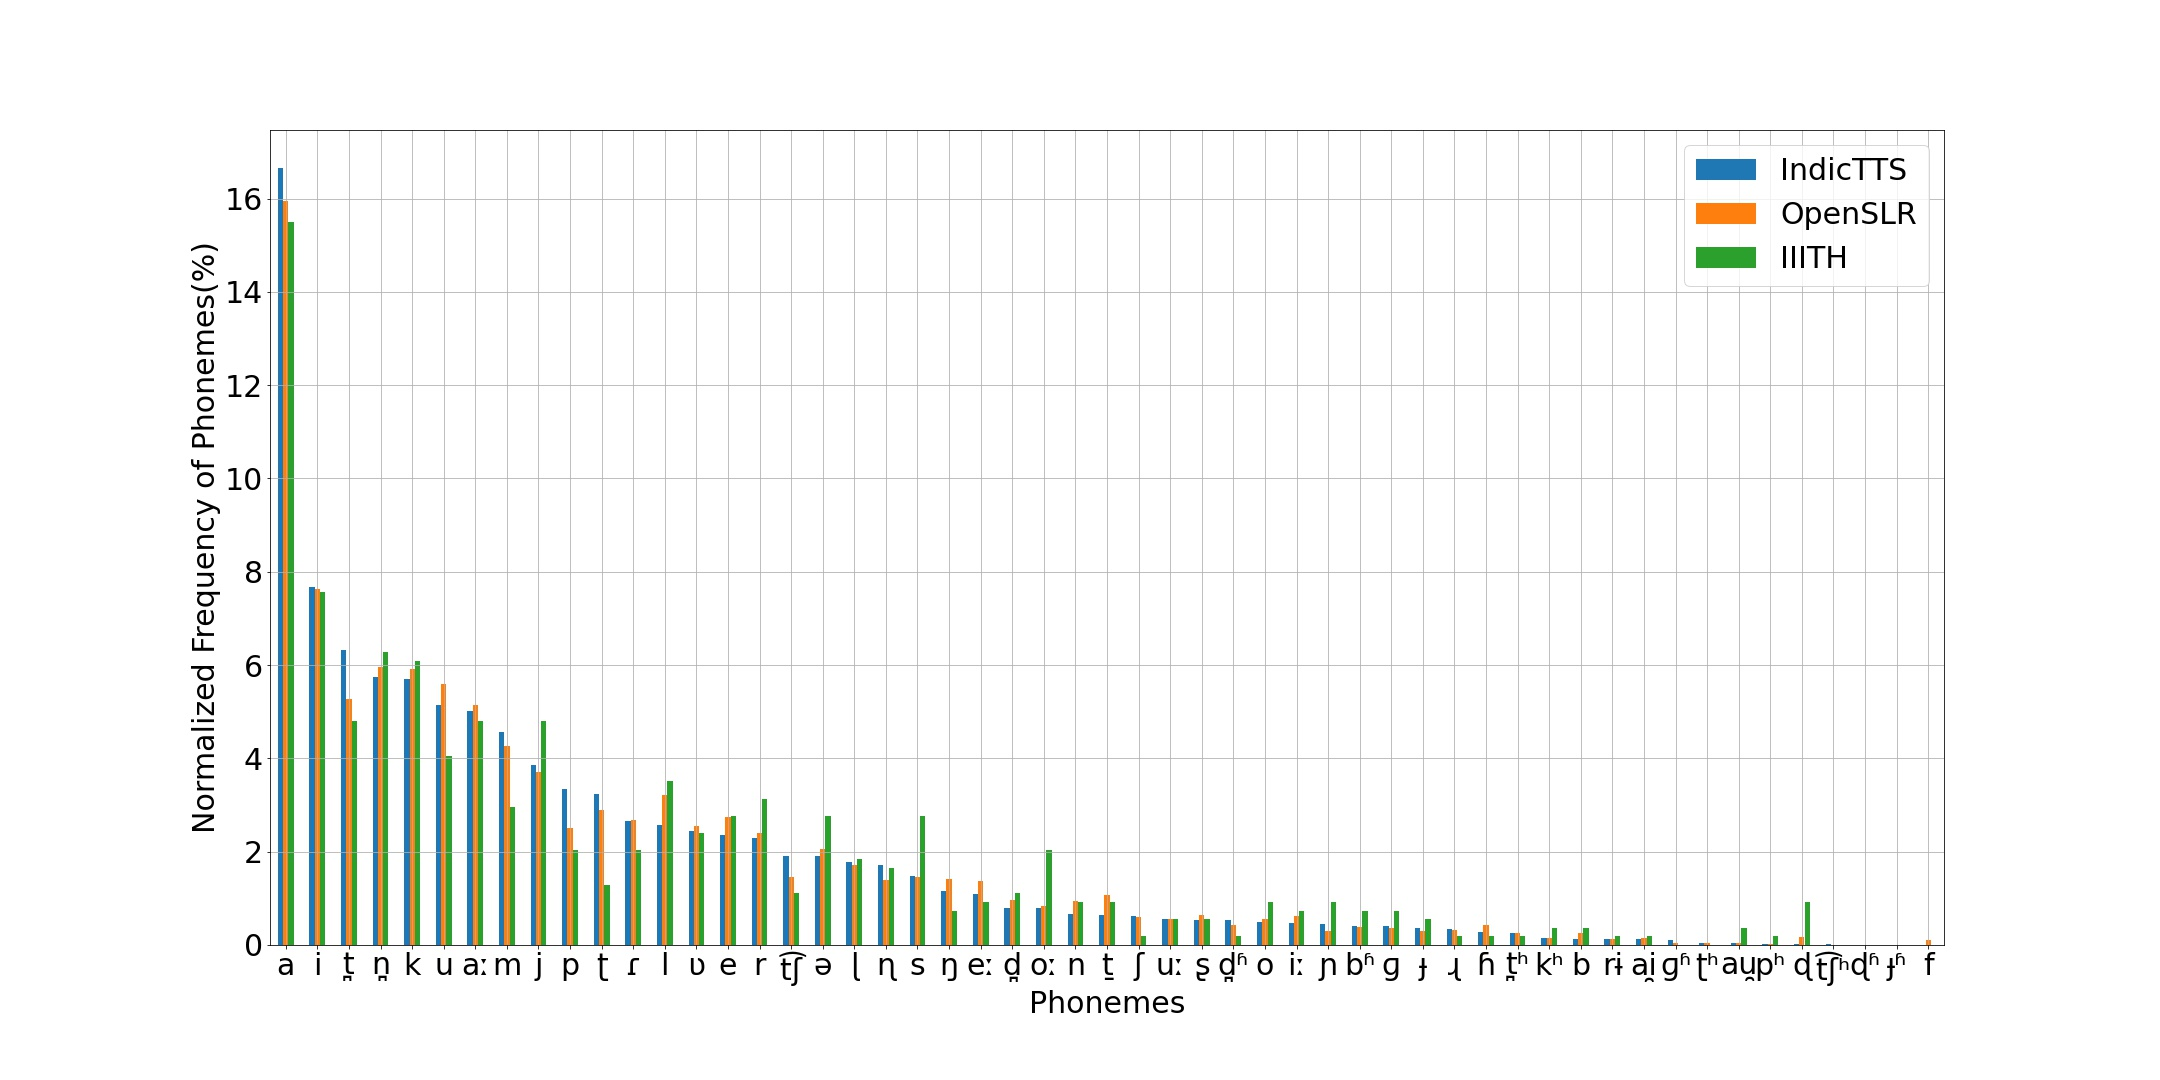
\includegraphics[width=\linewidth, trim=1cm 1cm 2cm 2cm,clip]{phoneticrichness.jpg}
	\caption{Phonemic diversity analysis of various speech corpora used in ASR Experiments. It indicates relative frequency of each phoneme.}
	% \Description{Phonemic diversity analysis of various speech corpora used in ASR Experiments. The graphs indicate all corpora are equally diverse.}
	\label{phoneticrichness}
\end{figure}

\subsection{Assisted Pronunciation Learning}

It is important for a new script learner to understand the pronunciations
correctly and get a comprehensive idea of phonetic features of the text. Mlphon
provides phonetic feature tags corresponding to every phoneme. A web
interface\footnote {Mlphon Web Interface \url{https://phon.smc.org.in/}} has
been developed for user friendly access to Mlphon features. As demonstrated in
Fig. \ref{fig:mlphon-web}, the graphical user interface accepts a word in Malayalam
script and provides syllabification, phonetic analysis and IPA transcription. This interface can aid even a non-native linguistic researcher to analyse and
understand the nuances of Malayalam script and pronunciation.

\begin{figure}[htpb]
	\centering
	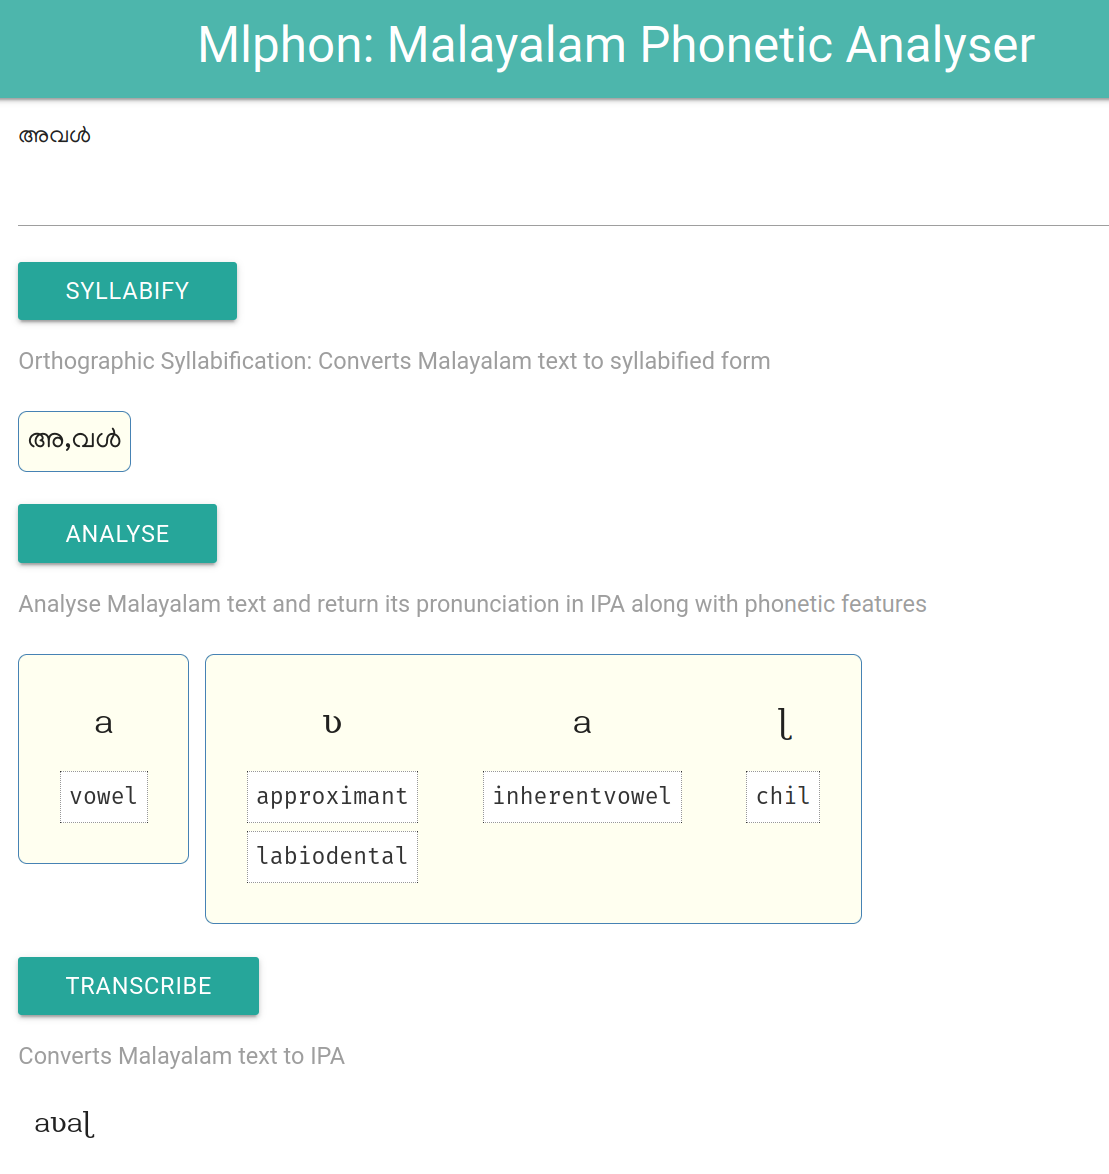
\includegraphics[width=0.6\textwidth]{mlphon-web.png}
	\caption{Web interface for Mlphon. Features of syllabification, phonetic analysis and IPA transcription are shown.}
	% \Description{Phonemic diversity analysis of various speech corpora used in ASR Experiments. The graphs indicate all corpora are equally diverse.}
	\label{fig:mlphon-web}
\end{figure}




\subsection{Text Sanity Check and Correction}

Large body of text (web crawled, crowd sourced, curated, transcribed or
annotated) is the backbone of training and testing modern NLP solutions of
large language models, part of speech taggers, text to speech and speech to
text systems. Mlphon can perform a script grammar check on the text corpora
under consideration and give pointers for manually correcting possibly corrupt
Malayalam text content due to presence of invisible characters, foreign
scripts, wrong script order etc.

% In the era of large language models being built on web crawled text corpora \cite{kunchukuttan2020ai4bharat}, it is necessary to ensure the sanity of text. Checking for the linguistic validity of character sequences can guarantee this to a large extent.


\begin{table}[htpb]
	\caption{Number of word tokens flagged as invalid by Mlphon on different transcribed speech corpus and corresponding error rates.}
	\label{tab:sanitycheck}
	\centering
	\begin{tabular}{lcc}
		\hline \hline
		Speech Corpora                                       & Error Count & Token Error Rate \\
		\hline
		Indic TTS \cite{baby2016resources}                   & 1013        & 1.2\%            \\
		OpenSLR \cite{he-etal-2020-open}                     & 83          & 0.3\%            \\
		Festvox IIITH \cite{prahallad2012iiit}               & 22          & 0.3\%            \\
		Indic Speech \cite{srivastava-etal-2020-indicspeech} & 4337        & 4.3\%            \\
		\hline
	\end{tabular}
\end{table}

The Table \ref{tab:sanitycheck} lists the number of tokens flagged as errors after
script grammar check using Mlphon in various Malayalam speech corpora. These
flagged errors were corrected before feeding them for training in ASR
experiments explained in chapter \ref{ch:lvcsr}. However, errors which do not
violate the script grammar rules can not be detected by Mlphon.


\subsection{Creation of Large Vocabulary Pronunciation Lexicon}

One of the  potential usages of Mlphon is its effectiveness in creating large vocabulary pronunciation lexicon efficiently. A detailed discussion on the creation of such a resource for Malayalam is discussed in Chapter \ref{ch:lvcsr} along with a comparison with similar tools qualitatively as well as quantitatively.

\section{Summary}


In this chapter, we presented a \gls{fst} based \gls{g2p} conversion system for Malayalam, called Mlphon. The system consists of three FSTs: a syllabifier FST, a phoneme analyser FST, and a G2P converter FST. We also described the various normalisation, tagging, and correction rules used in Mlphon to handle complex phonological processes in Malayalam, such as inherent vowel addition, alveolar conjuncts remapping, and dental nasal disambiguation.

Our intrinsic evaluation of Mlphon showed that the system achieved an accuracy of 99\% in syllabification and G2P conversion. We also discussed several potential applications of Mlphon, such as creating large vocabulary pronunciation lexicons, assisted pronunciation learning, and phonemic diversity analysis of speech corpora.

Overall, the development of Mlphon has contributed to the advancement of \gls{nlp} for Malayalam, and we believe that it can be further improved and expanded in the future to better serve the needs of researchers, developers, and users in the field.

% This chapter has presented the design and development of a bidirectional
% \gls{g2p} conversion tool Mlphon using \gls{fst} technology. The tool can also
% perform syllabification at orthographic level. The evaluation of this tool
% against a gold standard lexicon is presented. The various possible applications
% of this tool and a comparison with other automated lexicon creation tools is
% also presented in this chapter.